%!TEX program=pdflatex
\documentclass[8pt,xcolor={dvipsnames,table,xcdraw},handout]{beamer} % option aspectratio=169 for wide screen
\usetheme[
%%% options passed to the outer theme
    progressstyle=movCircCnt,   %either fixedCircCnt, movCircCnt, or corner
    rotationcw,          % change the rotation direction from counter-clockwise to clockwise
%    shownavsym          % show the navigation symbols
  ]{AAUsimple}
  
\usepackage[utf8]{inputenc}
\usepackage{csquotes}
\usepackage[english]{babel}
\usepackage[T1]{fontenc}
\usepackage{epigraph}
\usepackage{amsmath}
\usepackage{stmaryrd}
\usepackage[ruled]{algorithm2e}
\usepackage{caption}
\usepackage[absolute,overlay]{textpos}
\usepackage{hyperref}
\SetAlCapFnt{\small}
\SetAlCapNameFnt{\small}

\setbeamerfont{caption}{size=\scriptsize}
% colored hyperlinks
\newcommand{\chref}[2]{%
  \href{#1}{{\usebeamercolor[bg]{AAUsimple}#2}}%
}
\definecolor{colorAzulBienBonito}{RGB}{0,200,255}
\newcommand{\markdone}{\textcolor{PineGreen}{$\bullet$}}
\newcommand{\markonprogress}{\textcolor{colorAzulBienBonito}{$\bullet$}}
\newcommand{\markoff}{\textcolor{PineGreen}{$\circ$}}

\usepackage{booktabs}
\usepackage{makecell}
\usepackage{multicol}
\usepackage{multirow}
\usepackage{PTSans}
% \usepackage{array}
% \newcolumntype{L}[1]{>{\raggedright\let\newline\\\arraybackslash\hspace{0pt}}m{#1}}
% \newcolumntype{C}[1]{>{\centering\let\newline\\\arraybackslash\hspace{0pt}}m{#1}}
% \newcolumntype{R}[1]{>{\raggedleft\let\newline\\\arraybackslash\hspace{0pt}}m{#1}}


\title[Smart usage of context information for the analysis, design and generation of power-aware policies for MSAs]{Smart usage of context information for the analysis, design and generation of power-aware policies for mobile sensing apps}
         
\author[ITL Cinvestav-Tamaulipas]{Rafael Pérez Torres}

\institute[
  ITL Information Technology Laboratory\\
  Cinvestav\\
  Tamaulipas
] 
{Dr. César Torres Huitzil\\Dr. Hiram Galeana Zapién\\LTI Cinvestav}

\date{Doctoral seminar, 2017}

% specify a logo on the titlepage (you can specify additional logos an include them in institute command below
\pgfdeclareimage[height=1.5cm]{titlepagelogo}{cinvestav-logo/cinvestav-art-logo} % placed on the title page
\titlegraphic{\pgfuseimage{titlepagelogo}}

\setbeamersize{text margin left=5mm,text margin right=5mm} 
\graphicspath{ {../../../resources/images/} }

\begin{document}
% the titlepage
{\aauwavesbg%
\begin{frame}[plain,noframenumbering] % the plain option removes the header from the title page
  \titlepage
\end{frame}}

\begin{frame}{Structure}{}
  \tableofcontents[hideallsubsections]
\end{frame}

%!TEX root = ../slides.tex
\section{Introduction}
\subsection{Motivation}
\begin{frame}{Research background}{Motivation}
\begin{figure}[tb]
  \centering
  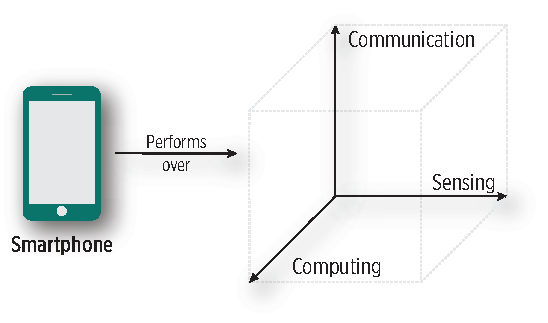
\includegraphics[width=0.4\textwidth]{vectors/smartphone-dimensions-v2}
  \caption{The advances in the communication, computing and sensing dimensions of mobile devices contribute to their acceptance by society~\cite{Islam2014}.}  
\end{figure}

\begin{block}{\small \textbf{Motivation}}
{
  \small
\begin{itemize}
  \item The sensing dimension enables \emph{context-awareness} in mobile devices, such as the smartphone.
  \item Battery advances are slower than those of other smartphone components~\cite{Kjaergaard2012}, growing 5-10\% yearly~\cite{Ma2012,Evarts2015}, a critical issue for the \textbf{mobile sensing applications}.
  % \item Battery advances are slower than those of other smartphone components~\cite{Kjaergaard2012}, growing 5-10\% yearly~\cite{Ma2012,Evarts2015}.
  % \item The energy constraint is critical for the continuous access to sensors required by \textbf{mobile sensing applications}. 
  \item Scientific efforts have been done for achieving the energy efficiency of the GPS location provider.
  \item The understanding of mobility could augment the location-awareness of the smartphone for many purposes, such as energy savings and the development of Mobility Based Services (MBSs).
  % \item As a high level of abstraction, mobility can be characterized as a sequence of frequently visited places (stay points).
\end{itemize}
}
\end{block}
\end{frame}

% \begin{frame}{Research background}{Motivation}
% \begin{block}{\small \textbf{Motivation}}
% {
%   \small
%    \begin{itemize}
%      \item For the sensing dimension, scientific efforts have been done for achieving the energy efficiency of the GPS location provider.
%      \item The understanding of mobility could augment the location-awareness of the smartphone for many purposes, such as energy savings and the development of Mobility Based Services (MBSs).
%      \item As a high level of abstraction, mobility can be characterized as a sequence of frequently visited places (a.k.a. stay points).
% \end{itemize}
% }
% \end{block}
% \end{frame}

\subsection{Research background}
%\subsection{Problem statement}
\begin{frame}{Research background}{Problem statement}
\small
\vspace{-0.5cm}
\begin{itemize}
  \item The understanding of mobility is possible at different spatial-temporal scales:
\end{itemize}

\begin{exampleblock}{\small \textbf{Fine-grain mobility patterns identification}}
 \begin{itemize}
    \item They refer to the transportation mode employed by user when moving between stay points.
    \item Given a set of values $\mathcal{V} = v_{acc~1},v_{acc~2},\ldots,v_{acc~n}$ obtained from accelerometer in the time interval $[t_1,t_2]$, identify fine-grain mobility information:
\begin{equation*}
  \text{\textbf{FineGrainMobilityIdentifier}}(\mathcal{V}) \rightarrow p_S \in \{ \text{static, walking, biking, vehicle} \}
\end{equation*}
with each $v_{acc~i} \in \mathcal{V}$ composed as $\langle acc_x,acc_y,acc_z,t \rangle$.
  \end{itemize} 
\end{exampleblock}

\begin{exampleblock}{\small \textbf{Coarse-grain mobility patterns identification}}
 \begin{itemize}
   \item They refer to motion at a large spatial scale related to user visiting stay points.
   \item \sloppy Given a set of values $\mathcal{V} = v_{gps~1},v_{gps~2},\ldots,v_{gps~n}$ obtained from GPS location provider in time interval $[t_1,t_2]$, identify coarse-grain mobility information:
\begin{equation*}
    \text{\textbf{CoarseGrainMobilityIdentifier}}(\mathcal{V}) \rightarrow p_S \in \{ \text{new stay point, arrival, departure} \}
\end{equation*}
with each $v_{gps~i} \in \mathcal{V}$ composed associated $\langle lat, lon, t \rangle$.
 \end{itemize}
\end{exampleblock}
\end{frame}


\begin{frame}{Research background}{Problem statement}
\small

\begin{exampleblock}{\small \textbf{Sensors sampling adaptation}}
\begin{itemize}
\item Given a set of coarse and fine-grain mobility patterns $\mathcal{P} = \{ p_{S_1}, p_{S_2}, \ldots, p_{S_n} \}$, and accuracy requirements of mobile app $req_{accuracy}$, implement a sampling policy for the adaptive duty cycling of sensors while reducing energy consumption:
\begin{equation*}
  \text{\textbf{PolicyGeneration}}( \mathcal{P}, req_{accuracy}) \longrightarrow{} \mathcal{S}_{conf}
\end{equation*}
where $\mathcal{S}_{conf} \rightarrow s, \mathcal{T}_{real}$ represents the sampling $\mathcal{T}_{real}$ that must be implemented for sensor $s$.
The $req_{accuracy}$ refers to the granularity of GPS sampling.
\end{itemize}
\end{exampleblock}

\begin{figure}[tb]
  \centering
  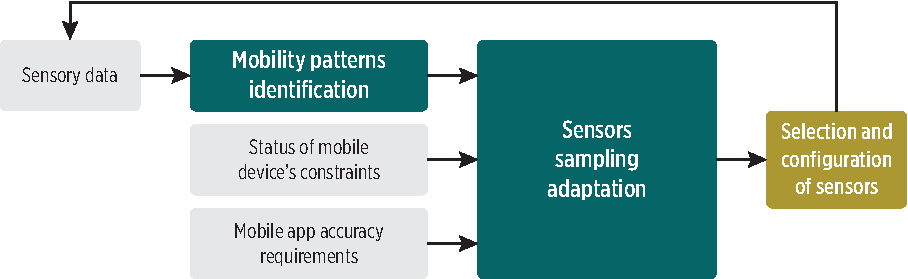
\includegraphics[width=0.7\textwidth]{vectors/problems-incorporation-v2}
  \caption{Interaction between problems.}
\end{figure}
\end{frame}

% \subsection{Hypothesis}
\begin{frame}{Research background}{Hypothesis}
\small
\begin{block}{\small \textbf{Hypothesis}}
\renewcommand{\baselinestretch}{1.4}
\begin{itemize}
  \item The energy consumption of continuous and extended location tracking could be reduced by means of a cognitive dynamic system that learns an expanded spatial-time model from mobility events detected from sensors data and that employs such model in a cognitive controller for dynamically adapting GPS sampling rate through sampling policies tailored to current mobility state.
\end{itemize}
\end{block}
\end{frame}


% \subsection{Objectives}
\begin{frame}{Research background}{Objectives}
\small
\begin{block}{\small \textbf{Main objective}}
\begin{itemize}
  \item To reduce the energy consumption of mobile sensing apps, which perform continuous sensor sampling, through self-adapting power-aware policies generated from context information obtained from sensors data.
\end{itemize}
\end{block}

\begin{block}{\small \textbf{Particular objectives}}
\begin{itemize}
  \item To detect mobility patterns from context information obtained from an inertial sensor (accelerometer) and location provider (GPS).
  \item To generate an accurate representation of detected patterns for summarizing user mobility.
  \item To dynamically adapt GPS sampling rate by means of a cognitive controller that employs the learned mobility representation and accuracy requirements for implementing power-aware sampling policies.
  \item To ease the development of mobile sensing applications that require user location tracking, i.e., LBSs and MBSs, isolating the complexity of sensors access and the associated efficient energy management.
\end{itemize}
\end{block}
\end{frame}



% \subsection{Methodology}
\begin{frame}{Research background}{Methodology}
\small
\begin{block}{\small \textbf{Methodology}}
\begin{enumerate}
  \item \textbf{Revision of state of the art power-aware sensing techniques.}
  \item \textbf{Formal definition and selection of mobility patterns to be identified.}
  \item \textbf{Research on algorithms for detecting mobility patterns.}
  \item \textbf{Design of the \emph{Mobility Events Detector}.}
  \item \textbf{Design of adaptive policies for energy efficient usage of sensors.}
  \item \textbf{Design of the Cognitive Controller.}
  \item \textbf{Development of a middleware involving the \emph{Mobility Events Detector} and the Cognitive Controller for the Android platform.}
  \item Experimentation in terms of spatial-time accuracy and energy efficiency.
\end{enumerate}
\end{block}
\end{frame}


\section{Problem statement}

\subsection{Preamble}

\begin{frame}{Problem description}
  \begin{block}{Current state of energy management}
    \begin{itemize}
      \item MSA access sensors in a continuous way over long periods of time.
      \item Sensors usage impacts directly on battery.
      \item Current smart devices' processors are designed to manage the heavy interaction with the user and the execution of mobile apps.
      \item A continuous sensor reading is out of their current objectives \citep{Priyantha2011}.
      % \item Current mobile platforms do not include mechanisms to perform periodical readings from sensors.
      \item API’s\footnote{API refers to Application Programming Interface.} by manufacturers only accomplish generic tasks like turning on – off sensors
    \end{itemize}
  \end{block}
\end{frame}

\begin{frame}{Problem description}
  \begin{block}{What do we need?}
    \begin{itemize}
      % \item API’s\footnote{API refers to Application Programming Interface.} by manufacturers only accomplish generic tasks like turning on – off sensors
      \item \textbf{High level information about user's context remains ignored}.
      \item A special framework to generate smart policies for continuous sensor access.
      \item This framework should consider:
        \begin{itemize}
          \item Mobile app requirements (e. g. the precision in the sensor data collection).
          \item Mobile device constraints (e. g. the current level of battery).
          \item Threshold values for performing a smart sensor usage (e. g. the lowest battery level for avoiding a permanent sensor usage).
        \end{itemize}
    \end{itemize}
  \end{block}
\end{frame}

\begin{frame}{Problem description}
  \begin{block}{A possible solution is}
    \begin{itemize}
      \item A policy is a high level concept that defines the usage sensors should observe to keep low energy consumption and fulfill mobile app requirements.

      \item The \emph{smartness} of policies is achieved by leveraging information about the user’s context obtained from sensors data.
      \begin{itemize}
        \item The user’s context can be recognized by employing a pattern identifier mechanism that is fed by raw data collected by sensors.

        \item The pattern becomes the descriptor of user’s context, and is the input for a policy generator mechanism that produces the policy to adapt the sensor usage, reduce the energy consumption and achieve mobile app objectives.
      \end{itemize}
      
    \end{itemize}
  \end{block}
\end{frame}


\subsection{Pattern identification}

\begin{frame}{Problem statement}
  \begin{exampleblock}{Pattern identification}
    Given a set $V = \left\{v_{1}, v_{2}, \dotsc, v_{n}\right\}$ of data values read from sensor $S$ in the time interval $T = \left\{t_{1}, t_{2}, \dotsc, t_{n}\right\}$, find the behavior pattern $Pattern_{S}$ that represents the activity of user.

    \begin{equation}
      PatternIdentifier( V ) \longrightarrow{} Pattern_{S} \in Patterns
    \end{equation}

    Where $Patterns$ is a set of patterns that represent an interesting state in the user activity.
  \end{exampleblock}
\end{frame}


\subsection{Policy generation}

\begin{frame}{Problem statement}
  \begin{exampleblock}{Policy generation}
    Given the pattern $Pattern_{S}$ detected in data from sensor $S$, parameters for assigning weight to energy $eh$ and precision $ph$, and physical constraints status $pc$ of a mobile device, find a policy to adapt the duty cycle of sensors.

    \begin{equation}
      PolicyGeneration( Pattern_{S}, eh, ph, pc ) \longrightarrow{} DutyCycle_{S}
    \end{equation}
  \end{exampleblock}
\end{frame}

\section{Hypothesis and objectives}


\subsection{Hypothesis}

\begin{frame}{Hypothesis}
  \begin{exampleblock}{Hypothesis}
    \begin{itemize}
      \item Smart policies generated through contextual information can be employed to reduce the energy consumption in a mobile device when performing continuous sensor readings.
    \end{itemize}    
  \end{exampleblock}
\end{frame}


\subsection{Objectives}

\begin{frame}{Objectives}
  \begingroup
    \setbeamercolor{block title}{bg=hsrmSec2Dark}
    \setbeamercolor{block body}{bg=hsrmSec2}
    
    \begin{block}{Main objective}
      \begin{itemize}
        \item Reduce energy consumption when performing continuous sensor readings in mobile devices by making use of context information.
      \end{itemize}
      
    \end{block}

    \begin{block}{Particular objectives}
      \begin{itemize}
        \item Identify behavior patterns which can provide meaningful context information from raw data collected by sensors.
        \item Generate smart policies for sensor usage from context information, mobile app requirements and mobile device constraints.
      \end{itemize}
    \end{block}
  \endgroup
\end{frame}

\section{Methodology}
\subsection{Methodology}
\begin{frame}{Methodology}
  \small
  \setbeamertemplate{enumerate item}{\Roman{enumi}}
  \begin{block}{Steps}
    \begin{enumerate}%[label=\bfseries Step \Roman*]
      %\renewcommand{\labelenumii}{Task \arabic{enumii}:}
      \item \textbf{Research on the characteristics of data delivered by sensors, in this case the GPS receiver.}

        % It can bring theoretical fundaments to improve the representation of data, for example achieving data compression.
        Identify special characteristics of GPS data that may trigger the study of techniques like outliers elimination, noise reduction, filtering, windowing, and framing to launch pre-processing of data delivered by sensors.

        % \begin{enumerate}
        %   \item Research on characteristics of data delivered by GPS receiver.
        % \end{enumerate}

      \item \label{itm:def-sel-mob-pttrns} \textbf{Definition and selection of mobility patterns to be identified.}

        This step is needed to identify the target mobility patterns that will be employed later in the pattern identifier element.

        % Examples of these mobility patterns are static, walking, running, vehicle at high speed, etc.

        The set of target mobility patterns defined here will be part of the input for the pattern identifier element.

        % \begin{enumerate}
        %   \setcounter{enumii}{1}
        %   \item Coding a sample app to gather GPS data from the smartphone.
        %   This app will access GPS receiver in a continuous and permanent way.
        %   \item Analysis of data delivered by the mobile app.
        %   \item Selection of the mobility patterns that will be recognized by the platform.
        %   \item Creation of the formal definition of mobility pattern.
        % \end{enumerate}
    \end{enumerate}
  \end{block}
\end{frame}

\begin{frame}{Methodology}
  \small
  \setbeamertemplate{enumerate item}{\Roman{enumi}}
  \begin{block}{Steps}
    \begin{enumerate}
      \setcounter{enumi}{2}
      \item \label{itm:research-alg-pttrn-rec} \textbf{Research and adaptation of algorithms to detect mobility patterns of user based on data delivered by GPS.}

        % Once the characteristics of data collected by sensors have been studied and the patterns to be identified have been defined, it is needed to detect a mobility pattern from these data.
        
        The pattern is helpful to get information about user's context and therefore in the generation of policies.
        
        The selected algorithms should consider the constraints present in mobile devices.

        % \begin{enumerate}
        %   \setcounter{enumii}{5}
        %   \item Research on algorithms for pattern recognition from GPS data.
        %   \item Definition of metrics for evaluating algorithms.
        %   \item Evaluation of algorithms.
        %   \item Selection of proper algorithm(s), discussing the best conditions for its (their) usage.
        % \end{enumerate}

      \item \textbf{Creation of the pattern identifier element (PIE).}

        This element must identify the pattern from data collected by sensors by employing the algorithm(s) selected in the Step \ref{itm:research-alg-pttrn-rec}.
        
        The pattern identified must be included in the set of mobility patterns defined in the Step \ref{itm:def-sel-mob-pttrns}.

        % \begin{enumerate}
        %   \setcounter{enumii}{9}
        %   \item Definition of parameters accepted by the PIE and their formal representation.
        %   \item Elaboration of the PIE.
        %   % \item Fine tunning of the PIE towards its usage in a constrained device (the smartphone)
        % \end{enumerate}

    \end{enumerate}
  \end{block}
\end{frame}

\begin{frame}{Methodology}
  \small
  \setbeamertemplate{enumerate item}{\Roman{enumi}}
  \begin{block}{Steps}
    \begin{enumerate}
      \setcounter{enumi}{4}

      \item \textbf{Creation of the policy generator element (PGE).}

        It includes the definition of a formal representation of policies.
        
        This policy generator element will obtain the duty cycle that the GPS receiver must implement to perform the next GPS reading.

        % \begin{enumerate}
        %   \setcounter{enumii}{11}
        %   \item Definition of parameters accepted by the PGE and their representation.
        %   \item Creation of the formal definition of \emph{policy}.
        %   \item Elaboration of the PGE.
        %   % \item Fine tunning of the PGE towards its usage in a constrained device (the smartphone)
        % \end{enumerate}

      \item \textbf{Development of a software element (SE) that integrates both PIE and PGE.}

        This software element will be implemented in the Android platform.
        
        % The Android platform is selected in this research because of its popularity, well documented SDK, and because its availability in the research center.

        % \begin{enumerate}
        %   \setcounter{enumii}{14}
        %   % \item Analysis and definition of logical elements involved in software abstractions.
        %   \item Definition of SE architecture.
        %   \item Research on Android API for specialized components related to sensor access and task-process management.
        %   \item Coding of the SE.
        % \end{enumerate}

      \item \textbf{Experimentation.}

        Key aspects are precision and energy saving.
        
        % Precision refers to the fidelity that data collected by employing policies maintain in relation to actual ground truth data.
        % This can be measured by executing data analysis processes over data collected by sensors through policies versus data collected without employing policies.
        
        % Energy saving refers to the reduction in the energy consumption that is obtained when applying policies versus the inter-built facilities of mobile operating systems.
        
        This step involves the definition of experiments and the development of mobile applications that employs the constructed software element.

        % \begin{enumerate}
        %   \setcounter{enumii}{17}
        %   \item Definition of experiments targeting energy saving and user tracking precision metrics.
        %   \item Development of mobile apps employing the SE for running the experimentation.
        %   \item Execution of the experimentation.
        %   \item Results analysis.
        % \end{enumerate}

    \end{enumerate}
  \end{block}
\end{frame}


\begin{frame}{Methodology}
  \begin{block}{Workflow of methodology}
    \begin{figure}
      \centering
      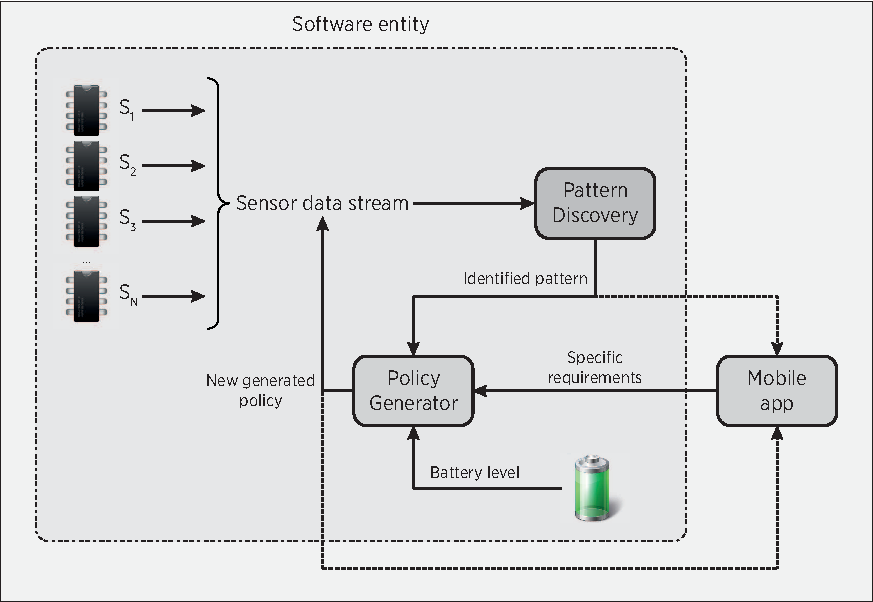
\includegraphics[scale=0.45]{methodology-stages}
      \caption[Methodology workflow]{Workflow described by the proposed methodology}
      \label{fig-methodology-workflow}
    \end{figure}
  \end{block}
\end{frame}

\section{Solution}
\subsection{Solution's overview}
{\aauwavesbg%
\begin{frame}[plain]
  \begin{textblock*}{8.5cm}(4.3cm,8.3cm)
  \small
  \textbf{Architecture of proposed system solution. The global perception-action cycle, the different memory types, and the internal feedback loops are observed.}
  \end{textblock*}

  \begin{textblock*}{1cm}(12cm,9.3cm)
  \scriptsize
  \insertframenumber~/~\inserttotalframenumber
  \end{textblock*}

  \centering
  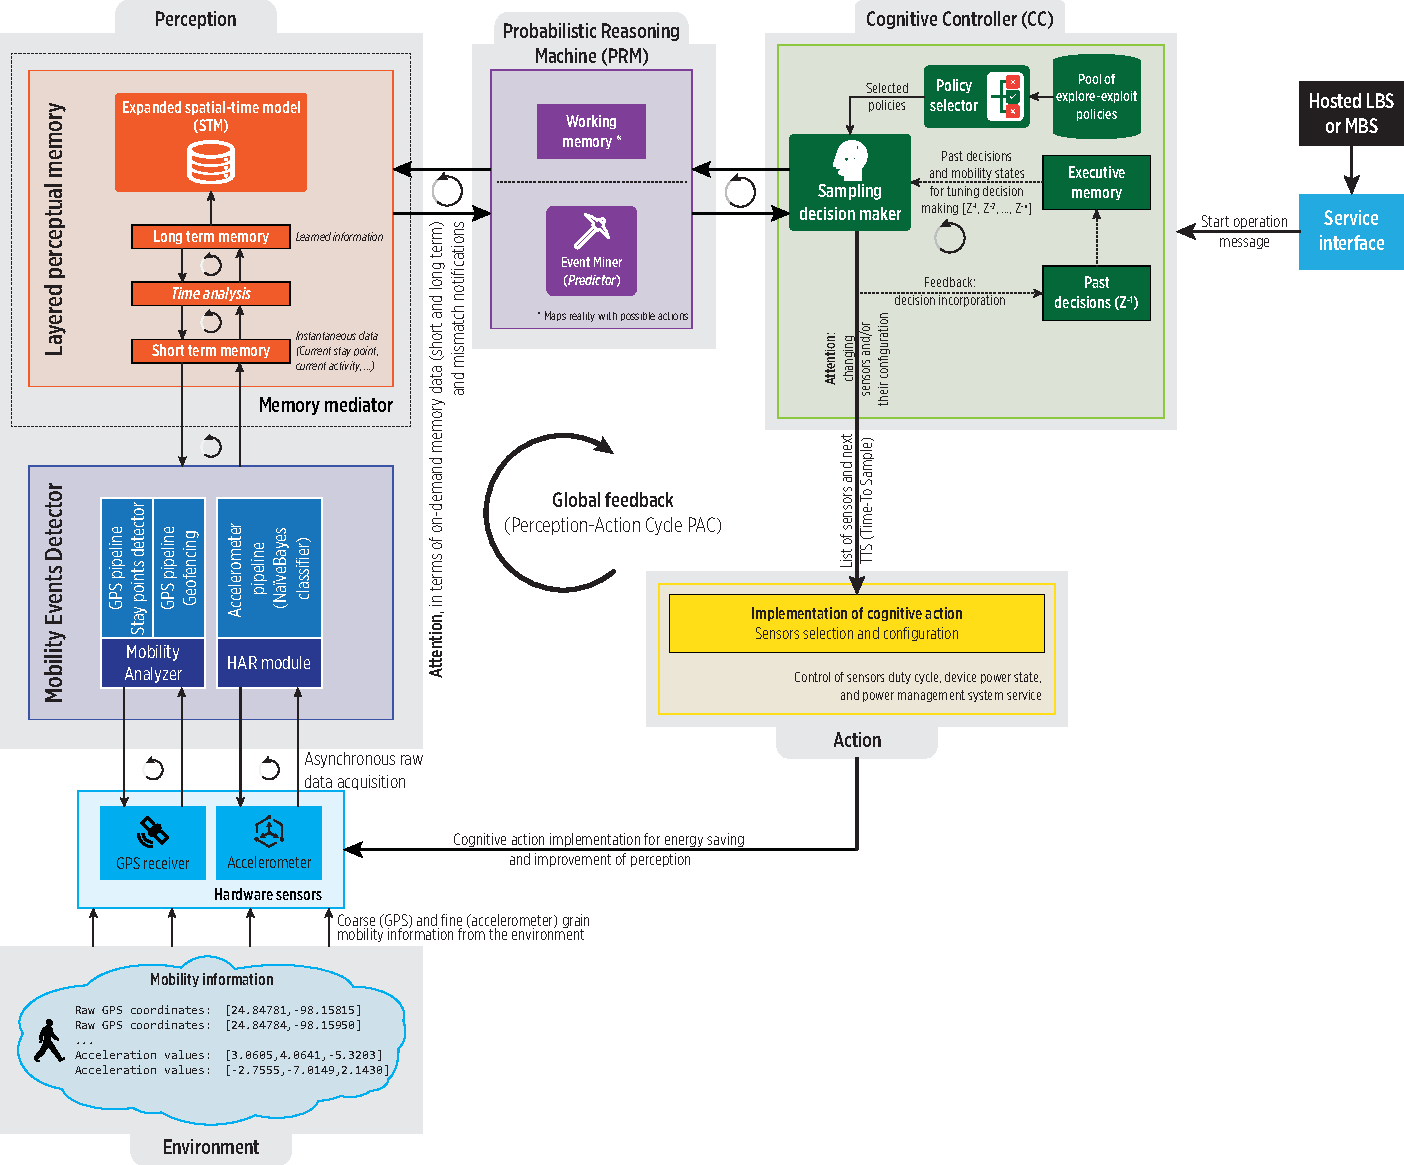
\includegraphics[width=0.98\textwidth]{vectors/inspired-cds-solution-for-slides}
  %\captionof{figure}{Architecture of proposed system solution. The global perception-action cycle and the internal loops are observed.}
\end{frame}}

% {\aauwavesbg
% \begin{frame}[plain]
%   \finalpage{
%     Thank you for your attention!
%   }
%   % { \tiny
%   %   \epigraph{\tiny We make our world significant by the courage of our questions and by the depth of our answers.}{\tiny \textit{Carl Sagan}}
%   % }
% \end{frame}}

\begin{frame}[allowframebreaks,noframenumbering]
        \frametitle{References}
%\bibliographystyle{plain}
{
\tiny{}
\bibliographystyle{unsrt}
\bibliography{../../../resources/references/library}
}
\end{frame}

\begin{frame}{Research background}{Contributions}
\small
\begin{block}{\small \textbf{Contributions}}
\begin{itemize}
  \item An on-device mobility patterns detector that works with streams of raw data collected by smartphone's sensors (GPS and accelerometer).
  \item An on-device mobility analyzer that incrementally builds a model of user mobility from the detected mobility patterns.
  \item A cognitive controller inspired on CDSs that, based on the mobility information learned, dynamically adapts GPS sampling rate through power-aware policies. 
  \item A middleware with the previous modules embedded for easing the development of LBSs and MBSs for the Android mobile platform.
\end{itemize}
\end{block}
\end{frame}

{\aauwavesbg%
  \begin{textblock*}{5cm}(0.3cm,0.3cm)
  \small
  \textbf{The architecture of the proposed system implemented in the Android software stack.}
  \end{textblock*}
\begin{textblock*}{1cm}(12cm,9.3cm)
  \scriptsize
  \insertframenumber~/~\inserttotalframenumber
  \end{textblock*}
\begin{frame}[plain]
  \centering
  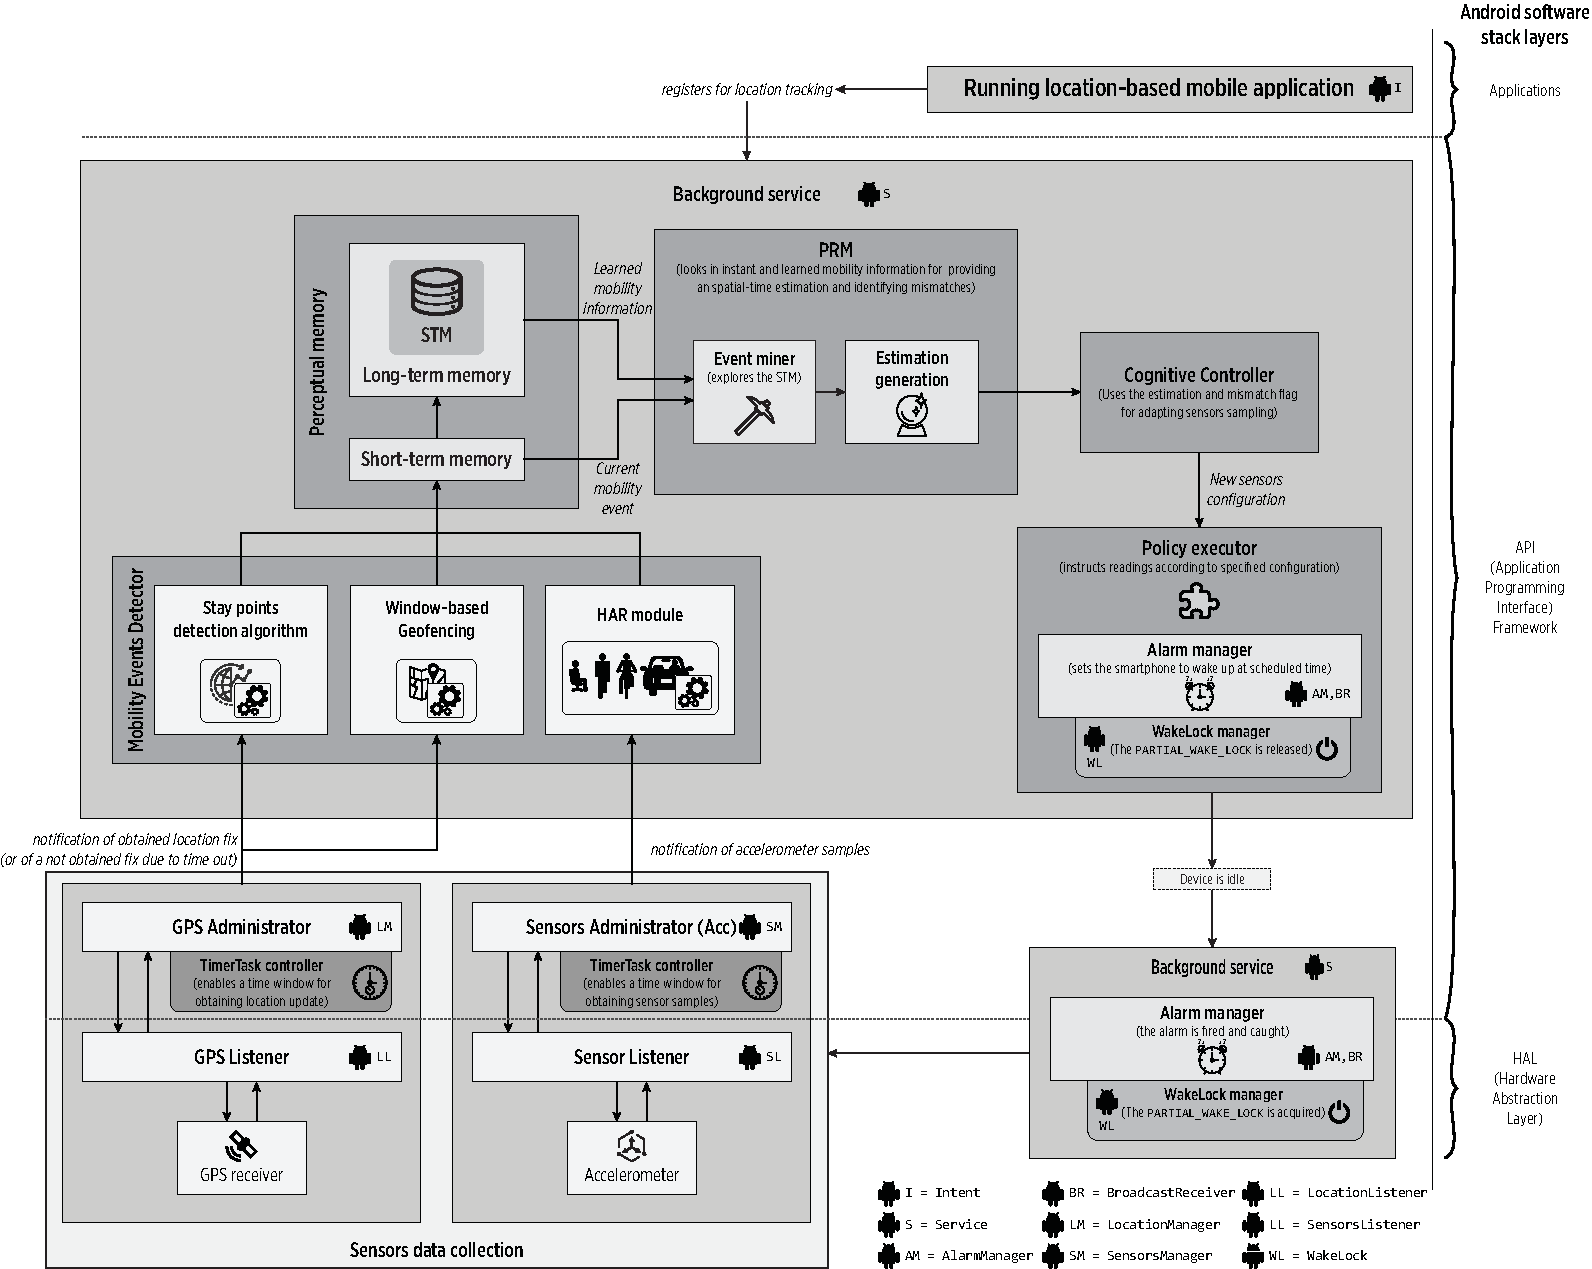
\includegraphics[width=\textwidth]{vectors/implementation}
\end{frame}}

\begin{frame}{Experimentation}{\emph{Stay Points Detector} module spatial-time accuracy: Results}
\vspace{-0.5cm}
\begin{table}
\centering
\renewcommand{\arraystretch}{0.8}
\resizebox{0.72\textwidth}{!}{%
\begin{tabular}{@{}lrrrrrr@{}}
\toprule
\multicolumn{1}{c}{\textbf{Trajectory}} & 
\multicolumn{1}{c}{\textbf{\begin{tabular}[c]{@{}c@{}}Sampling period\\(seconds)\end{tabular}}} & 
\multicolumn{1}{c}{\textbf{\begin{tabular}[c]{@{}c@{}}Live stay\\ points identified\end{tabular}}} & 
\multicolumn{1}{c}{\textbf{\begin{tabular}[c]{@{}c@{}}Average centroid\\ distance (meters)\end{tabular}}} & 
% \multicolumn{1}{c}{\textbf{\begin{tabular}[c]{@{}c@{}}Average diameter\\ distance (meters)\end{tabular}}} & 
% \multicolumn{1}{c}{\textbf{\begin{tabular}[c]{@{}c@{}}Average ST\\ difference (seconds)\end{tabular}}} & 
\multicolumn{1}{c}{\textbf{\begin{tabular}[c]{@{}c@{}}Average arrival\\ latency (seconds)\end{tabular}}} & 
\multicolumn{1}{c}{\textbf{\begin{tabular}[c]{@{}c@{}}Average departure\\ latency(seconds)\end{tabular}}} \\ 
\midrule
\multirow{6}{*}{Trajectory 1} 
 & 30 & 12 of 12 & 1.50 &   2.67 & 24.92 \\
 & 60 & 12 of 12 & 3.43 &   \textcolor{red}{\textbf{\emph{-12.33}}} & 17.42 \\
 & 90 & 12 of 12 & 4.04 &   15.17 & 32.42 \\
 & 120 & 12 of 12 & 6.66 &  \textcolor{red}{\textbf{\emph{-7.33}}} & 52.42 \\
 & 150 & 12 of 12 & 9.00 &  25.17 & 79.92 \\
 & 180 & 12 of 12 & 10.88 & 22.67 & 77.42 \\
 \cmidrule(l){1-6}

\multirow{6}{*}{Trajectory 2} 
 & 30 & 16 of 16 & 1.59 & 7.38 & 13.62 \\
 & 60 & 16 of 16 & 4.72 & 20.50 & 34.25 \\
 & 90 & 16 of 16 & 4.42 & 37.38 & 26.75 \\
 & 120 & 16 of 16 & 12.51 & 16.75 & 83.00 \\
 & 150 & 16 of 16 & 15.04 & \textcolor{red}{\textbf{\emph{-0.12}}} & 96.12 \\
 & 180 & 16 of 16 & 15.58 & 65.50 & 71.75 \\
 \cmidrule(l){1-6}

\multirow{6}{*}{Trajectory 3} 
 & 30 & 19 of 19 & 3.39 &  2.26 & 12.16 \\
 & 60 & 19 of 19 & 3.96 &  11.74 & 12.16 \\
 & 90 & 19 of 19 & 8.05 &  40.16 & 29.53 \\
 & 120 & 19 of 19 & 11.16  & 37.00 & 56.37 \\
 & 150 & 19 of 19 & 18.06  & 48.05 & 59.53 \\
 & 180 & 19 of 19 & \textcolor{green}{\textbf{22.52}} & 87.53 & 81.63 \\
 \cmidrule(l){1-6}

\multirow{6}{*}{Trajectory 4} 
 & 30 & 13 of 13 & 0.49 &  16.15 & 2.46 \\
 & 60 & 13 of 13 & 1.05 &  41.54 & 34.77 \\
 & 90 & 13 of 13 & 2.41 &  32.31 & 55.54 \\
 & 120 & 13 of 13 & 4.00 & 32.31 & 71.69 \\
 & 150 & 13 of 13 & 4.78 & 41.54 & 50.92 \\
 & 180 & 13 of 13 & 5.19 & 73.85 & 62.46 \\
 \cmidrule(l){1-6}

\multirow{6}{*}{Trajectory 5} 
 & 30 & 18 of 18 & 1.49 & 0.17 & 13.61 \\
 & 60 & 18 of 18 & 2.31 & 13.50 & 21.94 \\
 & 90 & 18 of 18 & 5.12 & \textcolor{red}{\textbf{\emph{-3.17}}} & 23.61 \\
 & 120 & 18 of 18 & 14.46 & 10.17 & \textcolor{red}{\textbf{\emph{-44.72}}} \\
 & 150 & 18 of 18 & 13.58 & 30.17 & \textcolor{red}{\textbf{\emph{-39.72}}} \\
 & 180 & 18 of 18 & 14.39 & 26.83 & \textcolor{red}{\textbf{\emph{-71.39}}} \\
 \cmidrule(l){1-6}

\multirow{6}{*}{Trajectory 6} 
 & 30 & 75 of 75 & 1.89 & 2.89 & 6.89 \\
 & 60 & \textcolor{blue}{\textbf{76 of 75}} & 3.54 & 8.49 & 24.89 \\
 & 90 & \textcolor{blue}{\textbf{76 of 75}} & 4.67  & 7.29 & 59.69 \\
 & 120 & \textcolor{blue}{\textbf{76 of 75}} & 6.71 & 29.29 & 77.69 \\
 & 150 & 75 of 75 & 9.33 & 42.89 & 113.29 \\
 & 180 & \textcolor{blue}{\textbf{76 of 75}} & 10.29 & 51.69 & 108.89 \\
 \bottomrule 
\end{tabular}
}
\caption{Spatial-time differences in detected stay points per sampling period (ST=stay time). The negative values in the ST difference and the arrival and departure latencies are caused by the combined effect of user mobility and sparse sampling rate on the \emph{StreamedZhen} algorithm, which generates stay points in subtly different coordinates with different time information.}
\end{table}
\end{frame}



\begin{frame}{Experimentation}{\emph{Geofencing} module spatial-time accuracy: Results}
\vspace{-0.5cm}
\begin{figure}
  \centering
  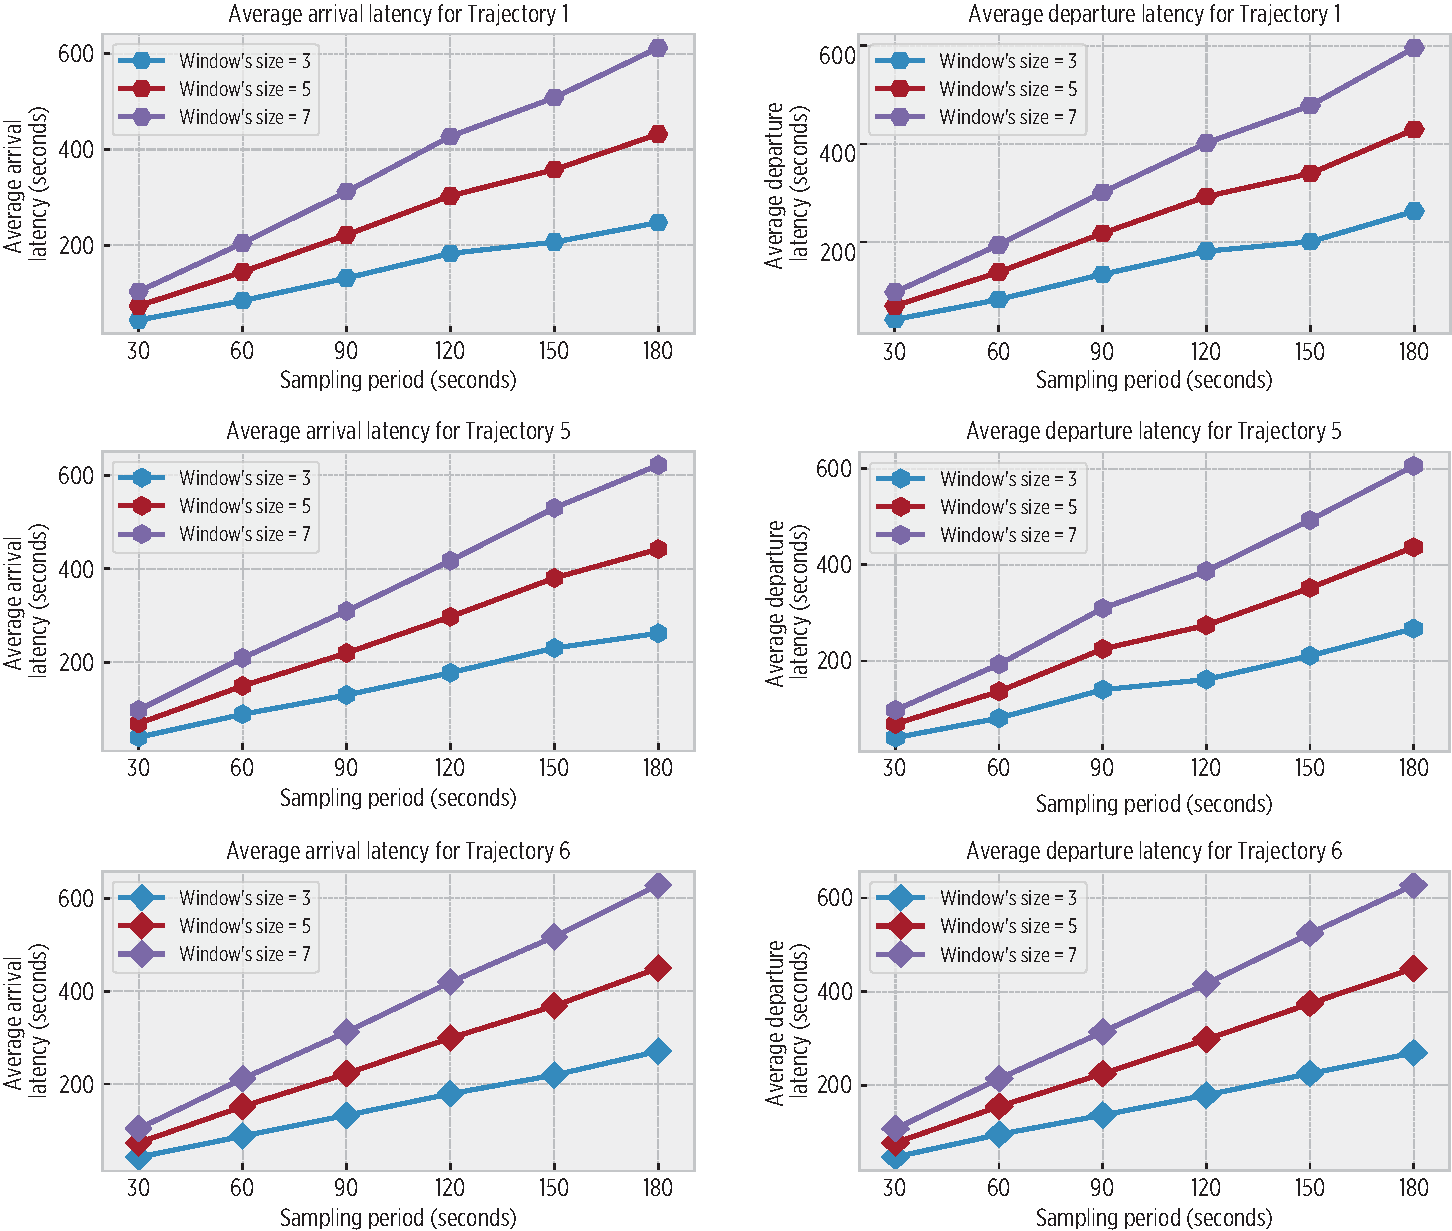
\includegraphics[width=0.75\textwidth]{vectors/experiments/exp-2/exp-2-latencies-for-slides}
  \caption{Arrival (left) and departure (right) latencies obtained by the Geofencing  module for each combination of sampling period and window length values. There is a tendency on the results as the shortest window’s sizes produce the shortest arrival latency values.}
\end{figure}
\end{frame}


\begin{frame}{Experimentation}{Holistic evaluation: Results}
\small 
\vspace{-0.5cm}
{
  \centering
  \includegraphics[width=0.7\textwidth]{vectors/experiments/exp-4/exp-4-sigmoid-header-top-row}
  \par 
}


\begin{columns}
\begin{column}[T]{0.5\textwidth}

\begin{block}{\small \textbf{Arrival distance difference}}
{
  \centering
  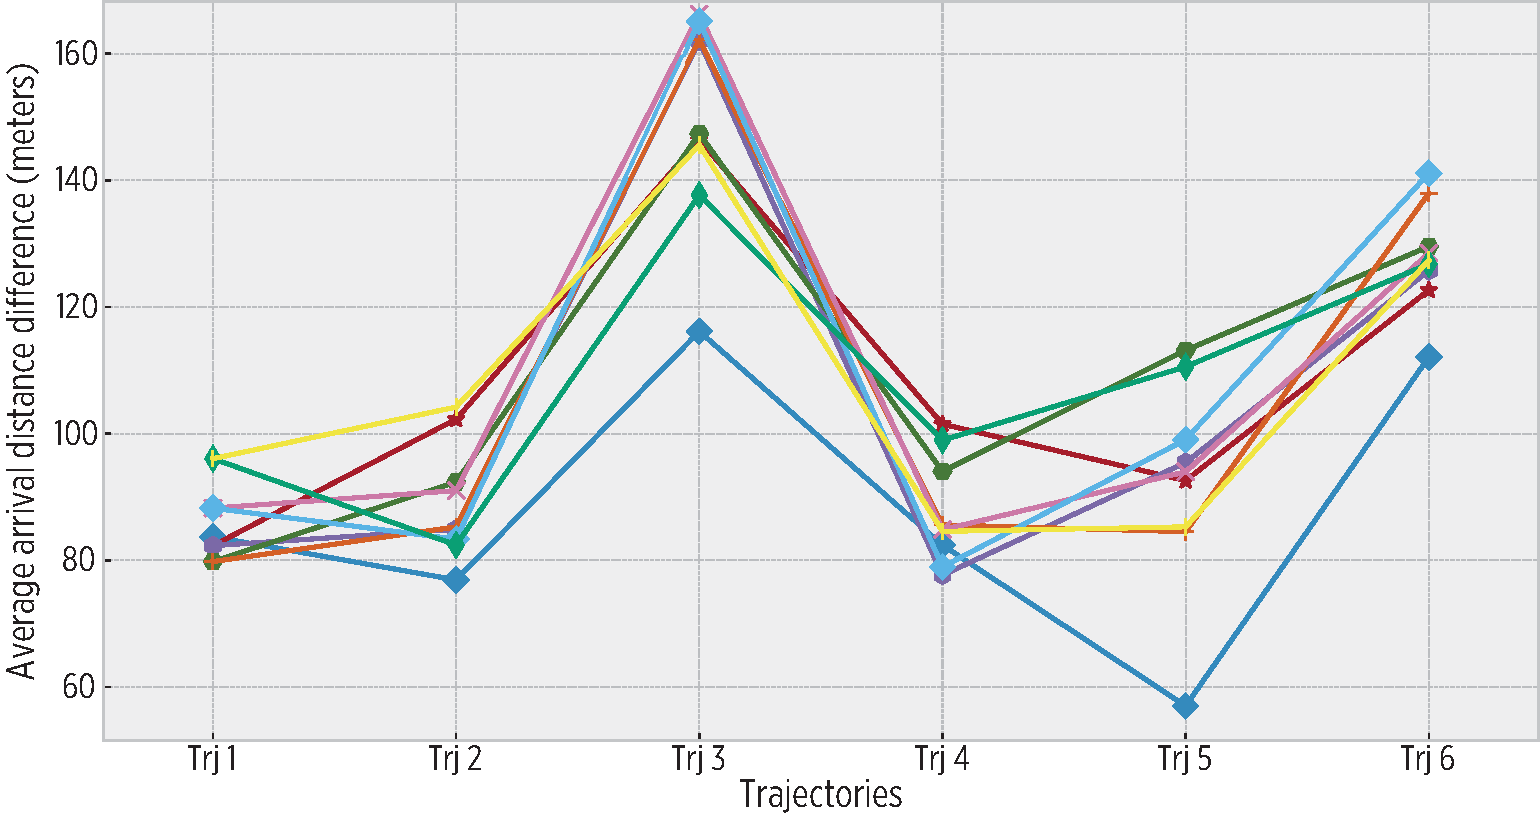
\includegraphics[width=\textwidth]{vectors/experiments/exp-4/exp-4-arrival-distance-for-slides-v2}
  \captionof{figure}{Arrival distance difference detected by the system throughout the different experimental trials. The values are shorter than for departure distance due to the decreasing speed that user describes when arriving to a stay point.}
  \par
}
\end{block}
\end{column}

\begin{column}[T]{0.5\textwidth}
\begin{block}{\small \textbf{Departure distance difference}}
{
  \centering
  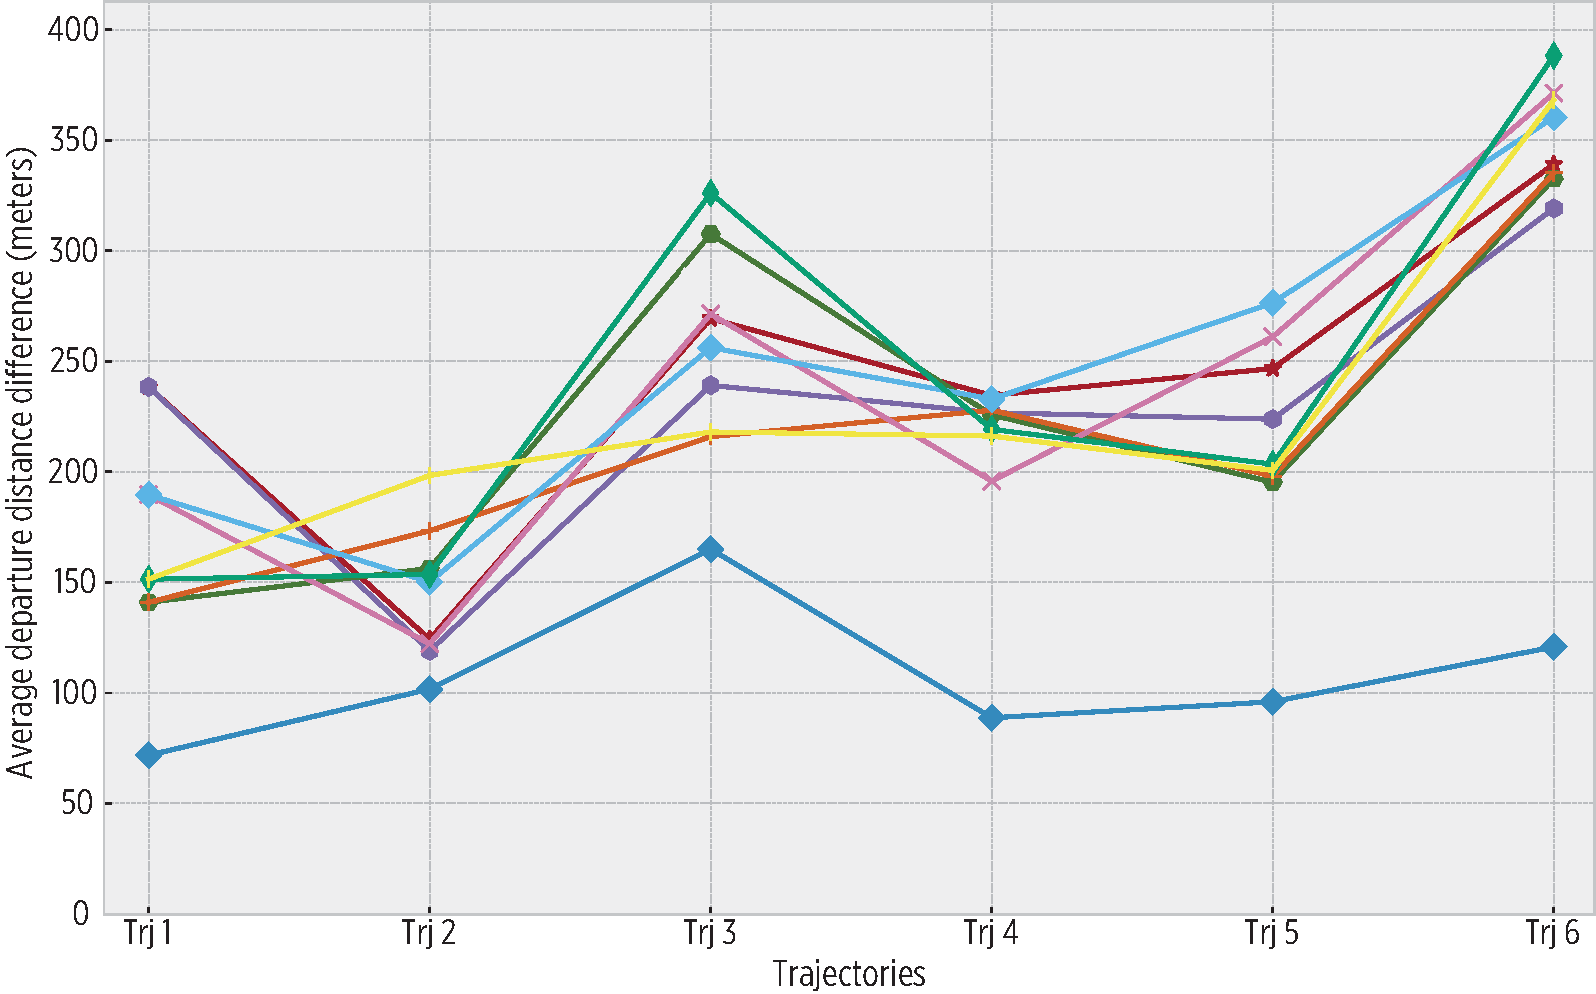
\includegraphics[width=\textwidth]{vectors/experiments/exp-4/exp-4-departure-distance-for-slides-v2}
  \captionof{figure}{Departure distance difference detected by the system throughout the different experimental trials. The larger distance differences are caused by the high speed with which user leaves the stay points (mostly using a vehicle as transportation mode).}
  \par
}
\end{block}

\end{column}
\end{columns}

\end{frame}


\begin{frame}{Experimentation}{Energy saving expectations of on-device stay points detection}
\small
% \vspace{-0.5cm}
\begin{columns}
\begin{column}{0.55\textwidth}
\begin{block}{\small \textbf{Description}}
\begin{itemize}
  \item This experiment explored whether a smartphone could detect stay points by itself, and the energy savings of such implementation with respect of typical Mobile Cloud Computing (MCC) based solutions.
  % \item Typical solutions implement a Mobile Cloud Computing (MCC) approach on which the smartphone only collects and offloads the processing to external servers.
\end{itemize}
\end{block}
\end{column}

\begin{column}{0.4\textwidth}
\begin{table}
\centering
\renewcommand{\arraystretch}{0.8}
\resizebox{0.95\textwidth}{!}{%
\begin{tabular}{lll}
\toprule
\multirow{2}{*}{\textbf{Stay Points Detector}} & \textbf{Time threshold} ($\delta_{time}$): & $45~min$ \\
\cmidrule[0.25pt]{2-3}
 & \textbf{Distance threshold} ($\delta_{distance}$): & $500~m$ \\

\cmidrule[0.25pt]{1-3}
\textbf{Sampling periods}: & \multicolumn{2}{l}{30, 60, 90, 120, 150 seconds} \\
\bottomrule
\end{tabular}
}
\caption{Input parameters for the energy saving expectations of on-device stay points detection experiment.}
\label{tab:exp-energy-performance-input-parameters}
\end{table}
\end{column}
\end{columns}

\begin{figure}
  \centering
  \includegraphics[width=\columnwidth]{vectors/local-poi-article/plot-energy-performance-r2-for-slides}
  \caption{Energy performance comparison of on-device vs. MCC sample apps using different GPS sampling periods. Each of the on-device trials last longer than its corresponding remote implementation.}
\end{figure}

\end{frame}


\begin{frame}{Experimentation}{Comparison with other solutions}
\begin{table}[]
\centering
\small
\renewcommand{\arraystretch}{1.2}
\begin{tabular}{@{}p{1cm}p{1.8cm}p{1.6cm}p{1.4cm}p{1cm}p{1cm}@{}}
\toprule
\textbf{Work} &
\textbf{Purpose} &
\textbf{Mobility type} &
\textbf{Involved sensors} &
\textbf{Trajectory tracking} &
\textbf{Place learning} \\ 
\midrule

\textbf{SenseLess} &
Location tracking &
Walking, static &
Accelerometer, GPS &
Yes &
No \\

\cmidrule[0.25pt]{1-6}
\textbf{SmartDC} &
Place tracking &
Not specified &
Cellular id, Wi-Fi, GPS&
No &
Yes \\

\cmidrule[0.25pt]{1-6}
Proposed system &
Location and place tracking &
Static, walking, biking, vehicle &
Accelerometer, GPS &
Yes &
Yes \\

\bottomrule
\end{tabular}%

\caption{Features comparison of proposed system and representative existing solutions.}
\end{table}
\end{frame}



% \begin{frame}[noframenumbering]{Detailed schedule}
% \begin{table}[]
% \centering
% \resizebox{0.95\textwidth}{!}{%
% \begin{tabular}{clccccccc}
%    &                                                                               & 2014 & \multicolumn{3}{c}{2015} & \multicolumn{3}{c}{2016}  \\
%    \cline{3-9}
% \multicolumn{2}{l}{\small{Work: \markdone~Done, \markonprogress~In progress, \markoff~To be done}} & 3rd & 1st & 2nd & 3rd & 1st & 2nd & 3rd \\
%    \toprule
% \multicolumn{2}{c}{\textsc{Step I}}                                                &  &  &  &  &  &  &  \\
% 1  & State-of-art reading                                                          & \markdone & \markdone &  &  &  &  &  \\
% 2  & State-of-art works categorization                                             &  & \markdone & \markdone  &  &  &  &  \\
% 3  & Documentation of information found (committee request)                        &  &  & \markdone &  &  &  &  \vspace{1em}\\

% \multicolumn{2}{c}{\textsc{Step II}}                                               &  &  &  &  &  &  &  \\
% 4  & \makecell[l]{Development of a mobile app for accelerometer and location \\data collection}    &  &  & \markdone & \markdone  &  &  &  \\
% 5  & Analysis of data                                                              &  &  &  & \markdone  &  &  &  \\
% 6  & Formal definition of mobility pattern                                         &  &  &  & \markdone &  &  &  \\
% 7  & Selection of mobility patterns                                                &  &  &  & \markdone & \markdone &  &  \vspace{1em}\\

% \multicolumn{2}{c}{\textsc{Step III}}                                              &  &  &  &  &  &  &  \\
% 8  & Research on classification algorithms for mobility patterns                   &  &  &  & \markdone & \markdone &  &  \\
% 9  & Definition of metrics for evaluating algorithms                               &  &  &  &  & \markdone &  &  \\
% 10 & Implementation of algorithms in mobile platform                               &  &  &  &  & \markdone & \markdone  &  \\
% 11 & Selection of best algorithms according to metrics                             &  &  &  &  &  & \markdone &  \vspace{1em}\\

% \multicolumn{2}{c}{\textsc{Step IV}}                                               &  &  &  &  &  &  &  \\
% 12 & Definition and modeling of parameters needed by the \emph{Mobility Events Detector}                       &  &  &  & \markdone & \markdone & \markdone & \markdone \\
% 13 & Development of the \emph{Mobility Events Detector}.  &  &  &  & \markdone & \markdone & \markdone & \markdone \\
% \bottomrule
% \end{tabular}%
% }
% \caption{Schedule of activities (each column represents a four months period)}
% \end{table}
% \end{frame}

% \begin{frame}[noframenumbering]{Detailed schedule}
% \begin{table}[]
% \centering
% \resizebox{0.95\textwidth}{!}{%
% \begin{tabular}{clccccccc}
%    &                                                                               & \multicolumn{3}{c}{2016} & \multicolumn{3}{c}{2017} & 2018 \\
%    \cline{3-9}
% \multicolumn{2}{l}{\small{Work: \markdone~Done, \markonprogress~In progress, \markoff~To be done}}   & 1st & 2nd & 3rd & 1st & 2nd & 3rd & 1st \\
%    \toprule
% \multicolumn{2}{c}{\textsc{Step V}}                                                &  &  &  &  &  &  & \\
% 14  & Formal definition of policy                                                  &  &  & \markdone &  &  &  & \\
% 15  & \makecell[l]{Research and evaluation of techniques for\\generation and adaption of policies}&  &  & \markdone & \markdone  &  &  & \\
% 16  & Design and execution of experiments applied to use cases                     &  &  & \markdone & \markdone  &  &  & \\
% 17  & Selection of policies                                                        &  &  &  & \markdone  &  &  & \vspace{1em} \\

% \multicolumn{2}{c}{\textsc{Step VI}}                                               &  &  &  &  &  &  & \\
% 18  & Definition and modeling of Cognitive Controller parameters                                    &  &  &  &  & \markdone  &  & \\
% 19  & Development of the Cognitive controller                                                          &  &  &  &  & \markdone  &  & \vspace{1em} \\

% \multicolumn{2}{c}{\textsc{Step VII}}                                               &  &  &  &  &  &  & \\
% 20  & Analysis of components into software abstractions                             &  &  &  &  & \markdone  &  & \\
% 21  & Research on Android API for specialized components                            &  &  &  &  & \markdone  &  & \\
% 22  & Development of middleware                                                     &  &  &  &  & \markdone  &  & \vspace{1em}\\

% \multicolumn{2}{c}{\textsc{Step VIII}}                                              &  &  &  &  &  &  & \\
% 23  & \makecell[l]{Definition of experiments aimed at accuracy\\and energy consumption metrics}    &  &  &  &  &  & \markdone & \\
% 24  & Development of experimental sample mobile apps                                &  &  &  &  &  & \markonprogress & \\
% 25  & Experiments execution                                                         &  &  &  &  &  & \markonprogress & \markoff  \\
% 26  & Final results analysis                                                              &  &  &  &  &  &  & \markoff \\
% \bottomrule
% \end{tabular}%
% }
% \caption{Schedule of activities (each column represents a four months period)}
% \end{table}
% \end{frame}

% \begin{frame}[noframenumbering]{Detailed schedule}
% \begin{table}
% \centering
% \resizebox{\textwidth}{!}{%
% \begin{tabular}{clcccccccccccc}
%    &                                                                               & 2014 & \multicolumn{3}{c}{2015} & \multicolumn{3}{c}{2016} & \multicolumn{3}{c}{2017} & \multicolumn{2}{c}{2018} \\
%    \cline{3-14}
%  \multicolumn{2}{l}{\small{Work: \markdone~Done, \markonprogress~In progress, \markoff~To be done}} & 3rd & 1st & 2nd & 3rd & 1st & 2nd & 3rd & 1st & 2nd & 3rd & 1st & 2nd\\
%    \toprule
% \multicolumn{2}{c}{\textsc{Required tasks}}                                        &  &  &  &  &  &  &  &  &  &  &  & \\
% A   & Related courses                                                              & \markdone  & \markdone  & \markdone &  &  &  &  &  &  &  &  & \\
% B   & Research articles submission                                                 &  &  &  & \markdone &  & \markdone &  &  &  &  & \markonprogress & \\
% C   & Predoctoral exam preparation                                                 &  &  &  &  &  &  &  &  & \markdone &  &  & \\
% D   & Thesis writing                                                               & \markdone  &  &  & \markdone &  &  & \markdone &  &  & \markonprogress & \markoff & \markoff \\

% \bottomrule
% \end{tabular}%
% }
% \caption{Schedule of required activities}
% \end{table}
% \end{frame}


% \begin{frame}[noframenumbering]{Layered perceptual memory}{Short and long-term memory information}
% \vspace{-0.25cm}
% \small
% \begin{block}{\small \textbf{Layered perceptual memory}}
% \begin{itemize}
%     \item Short-term memory information: current (observed) mobility status.
%     \item Long-term memory information: the Expanded Spatial-Time model (STM).
% \end{itemize}
% \end{block}

% \begin{block}{\small \textbf{Expanded Spatial-Time model}}
% \begin{itemize}
%   \item The highest level of mobility information held by the system.
% \end{itemize}
% {
%   \centering
%   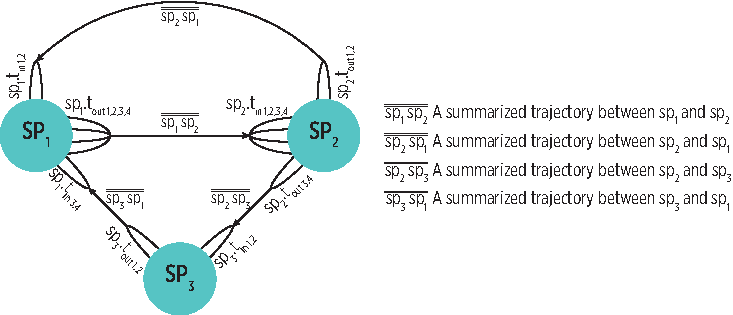
\includegraphics[width=0.75\textwidth]{vectors/stm-slides}
%   \captionof{figure}{A conceptual representation of the STM's structure.}
% \par }
% \end{block}
% \end{frame}

% \begin{frame}[noframenumbering]{Layered perceptual memory}{Expanded Spatial-Time model (STM)}
% \small
% \begin{block}{\small \textbf{Generation of the STM}}
% \begin{itemize}
%     \item Incrementally built with the coarse-grain mobility events detected by the \emph{Mobility Events Detector}.
% \end{itemize}
% {
%   \centering
%   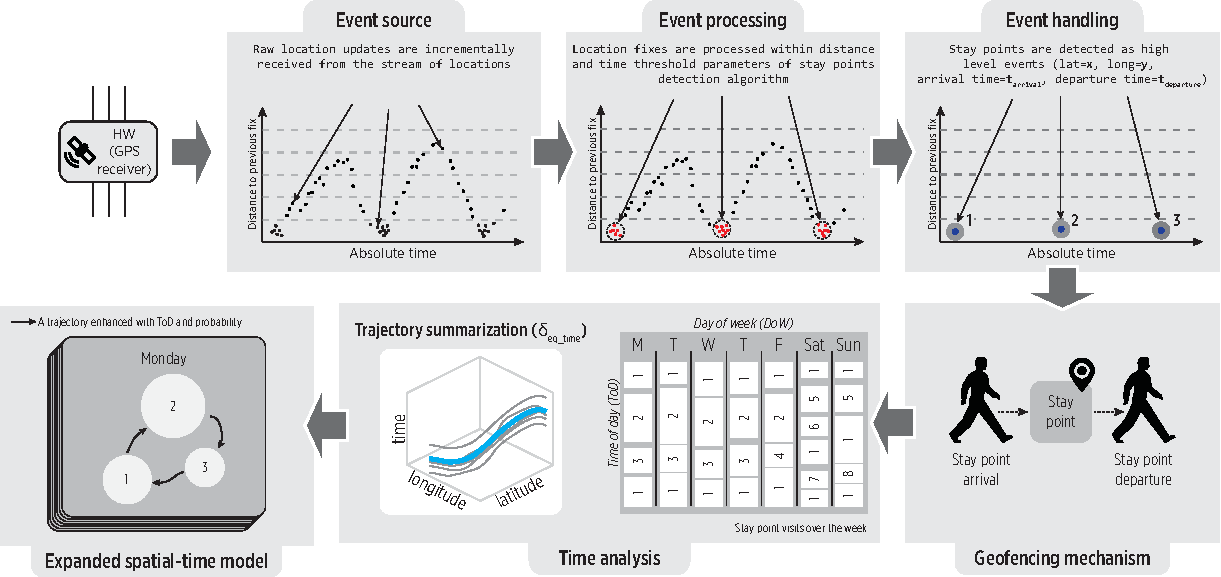
\includegraphics[width=\textwidth]{vectors/event-driven-memory-generation-for-slides}
%   \captionof{figure}{A conceptual representation of the steps for generating the STM from raw sensors data.}
%   \par
% }
% \end{block}
% \end{frame}


% \begin{frame}[noframenumbering]{Cognitive controller (CC)}{Description}
% \small
% \vspace{-0.5cm}
% \begin{columns}
% \begin{column}[T]{0.5\textwidth}
% \begin{block}{\small \textbf{Goals}}
%   \begin{itemize}
%       \item To reduce the energy consumption of location tracking by relying on PRM's estimations.
%       \item To reduce the system uncertainty about current user mobility.
%   \end{itemize}
% \end{block}
% \end{column}

% \begin{column}[T]{0.5\textwidth}
% \begin{block}{\small \textbf{Possible cognitive actions}}
%   \begin{itemize}
%     \item \textbf{Exploitation policies}: When system uncertainty is low for saving energy purposes.
%     \item \textbf{Exploration policies}: When system uncertainty is high for recovering for accuracy loss.
%   \end{itemize}
% \end{block}
% \end{column}
% \end{columns}

% \begin{figure}
%   \centering
%   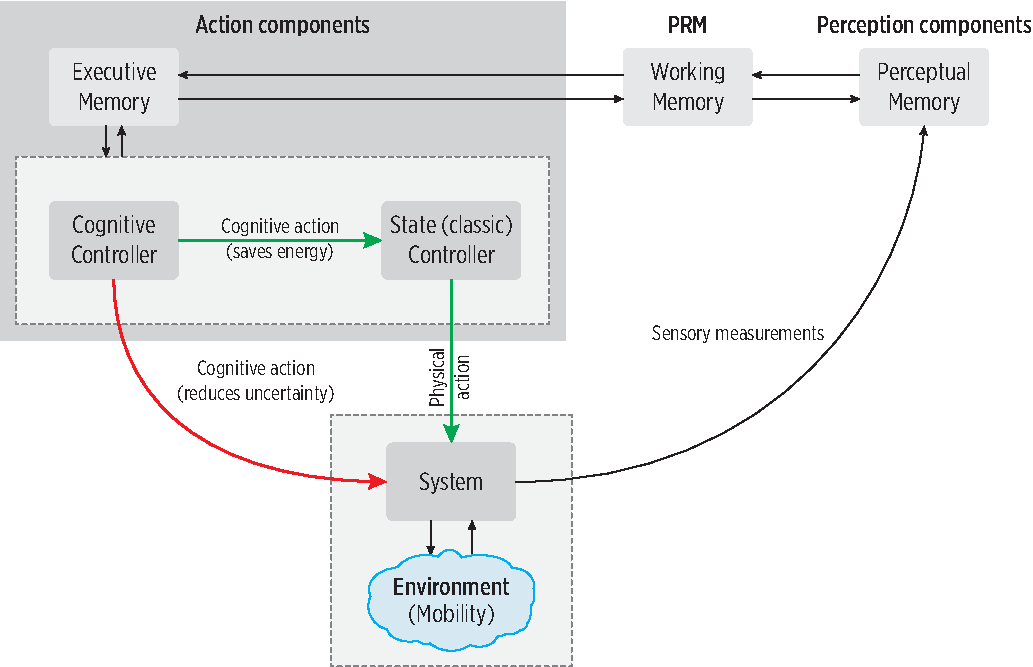
\includegraphics[width=0.65\textwidth]{vectors/cognitive-controller-architecture}
%   \caption{A generic cognitive controller architecture}
% \end{figure}
% \end{frame}

% \begin{frame}[noframenumbering]{Cognitive controller}{Policies tailored for user mobility}
% \small
% \begin{block}{\small \textbf{Stay point mode}}
%   \begin{itemize}
%       \item A sampling based on the sigmoid function $sig(x) = \frac{1}{1+e^{-\alpha x}}$ as a model for the mobility phase transitions.
%       \item Higher sampling rate on arrival and departure, when the user is more likely to move, and slower at the middle of a visit.
%   \end{itemize}
% \end{block}

% \begin{columns}
% \begin{column}{0.45\textwidth}
% \begin{figure}
%   \centering
%   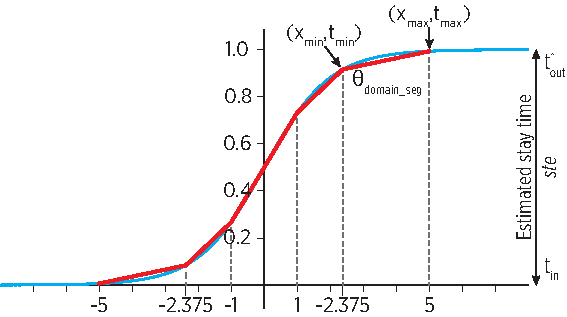
\includegraphics[width=0.99\linewidth]{vectors/sigmoid-segmentation-for-slides}
%   \caption{Approximation of the sigmoid through straight segments.}
% \end{figure}
% \end{column}

% \begin{column}{0.55\textwidth}
% \begin{figure}
%   \centering
%   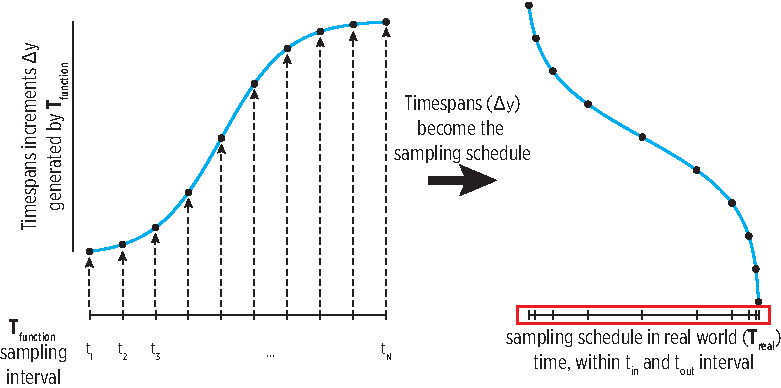
\includegraphics[width=0.99\linewidth]{vectors/sigmoid-driven-sampling-policy-for-slides}
%   \caption{A snapshot of the process for producing a sigmoid sampling.}
% \end{figure}
% \end{column}
% \end{columns}
% \end{frame}

% \begin{frame}[noframenumbering]{Preliminary experimentation}{\emph{Stay Points Detector} module spatial-time accuracy}
% \small

% \begin{columns}
% \begin{column}[T]{0.55\textwidth}

% \begin{block}{\small \textbf{Description}}
% \begin{itemize}
%   \item This experiment evaluates the spatial-time accuracy of the \emph{Stay Points Detector} module under different GPS sampling rates in terms of centroid distances and latencies.
% \end{itemize}
% \end{block}

% \end{column}
% \begin{column}[T]{0.45\textwidth}
% \begin{table}
% \centering
% \renewcommand{\arraystretch}{0.6}
% \resizebox{0.9\textwidth}{!}{%
% \begin{tabular}{lll}
% \toprule
% \multirow{2}{*}{\textbf{Stay Points Detector}} & \textbf{Time threshold} ($\delta_{time}$): & $45~min$ \\
% \cmidrule[0.25pt]{2-3}
%  & \textbf{Distance threshold} ($\delta_{distance}$): & $500~m$ \\

% \cmidrule[0.25pt]{1-3}
% \textbf{Sampling periods}: & \multicolumn{2}{l}{30, 60, 90, 120, 150, 180 seconds.} \\

% \cmidrule[0.25pt]{1-3}
% \textbf{Trajectories}: & \multicolumn{2}{l}{All ground truth trajectories.} \\
% \bottomrule
% \end{tabular}
% }
% \caption{Input parameters for the spatial-time accuracy of stay points experiment.}
% \end{table}
% \end{column}
% \end{columns}

% \vspace{-0.5cm}
% \begin{block}{\small \textbf{Results}}
% \begin{columns}
% \begin{column}{0.65\textwidth}
% \begin{figure}
%   \centering
%   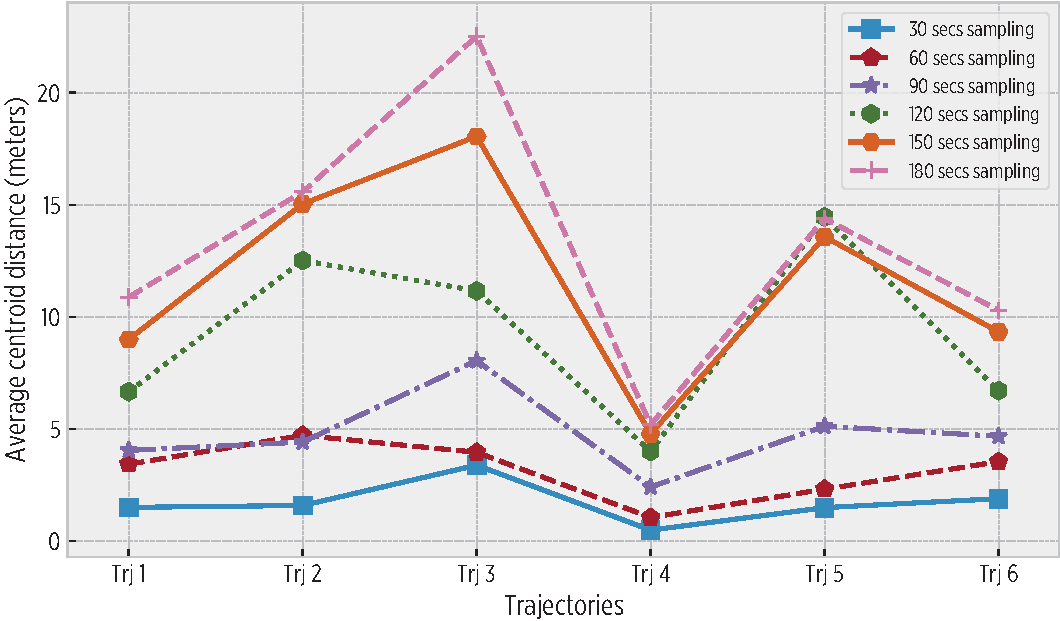
\includegraphics[width=0.99\textwidth]{vectors/exp-1-centroid-distance}
% \end{figure}
% \end{column}
% \begin{column}{0.3\textwidth}
% \captionof{figure}{The impact of different sampling periods on the centroid distance of identified stay points in each trajectory. A maximum centroid distance of $22.52~m$ is identified when employing the 180 seconds sampling period.}
% \end{column}
% \end{columns}

% \end{block}
% \end{frame}


% \begin{frame}[noframenumbering]{Preliminary experimentation}{\emph{Geofencing} module spatial-time accuracy: Results}
% \vspace{-0.5cm}
% \begin{figure}
%   \centering
%   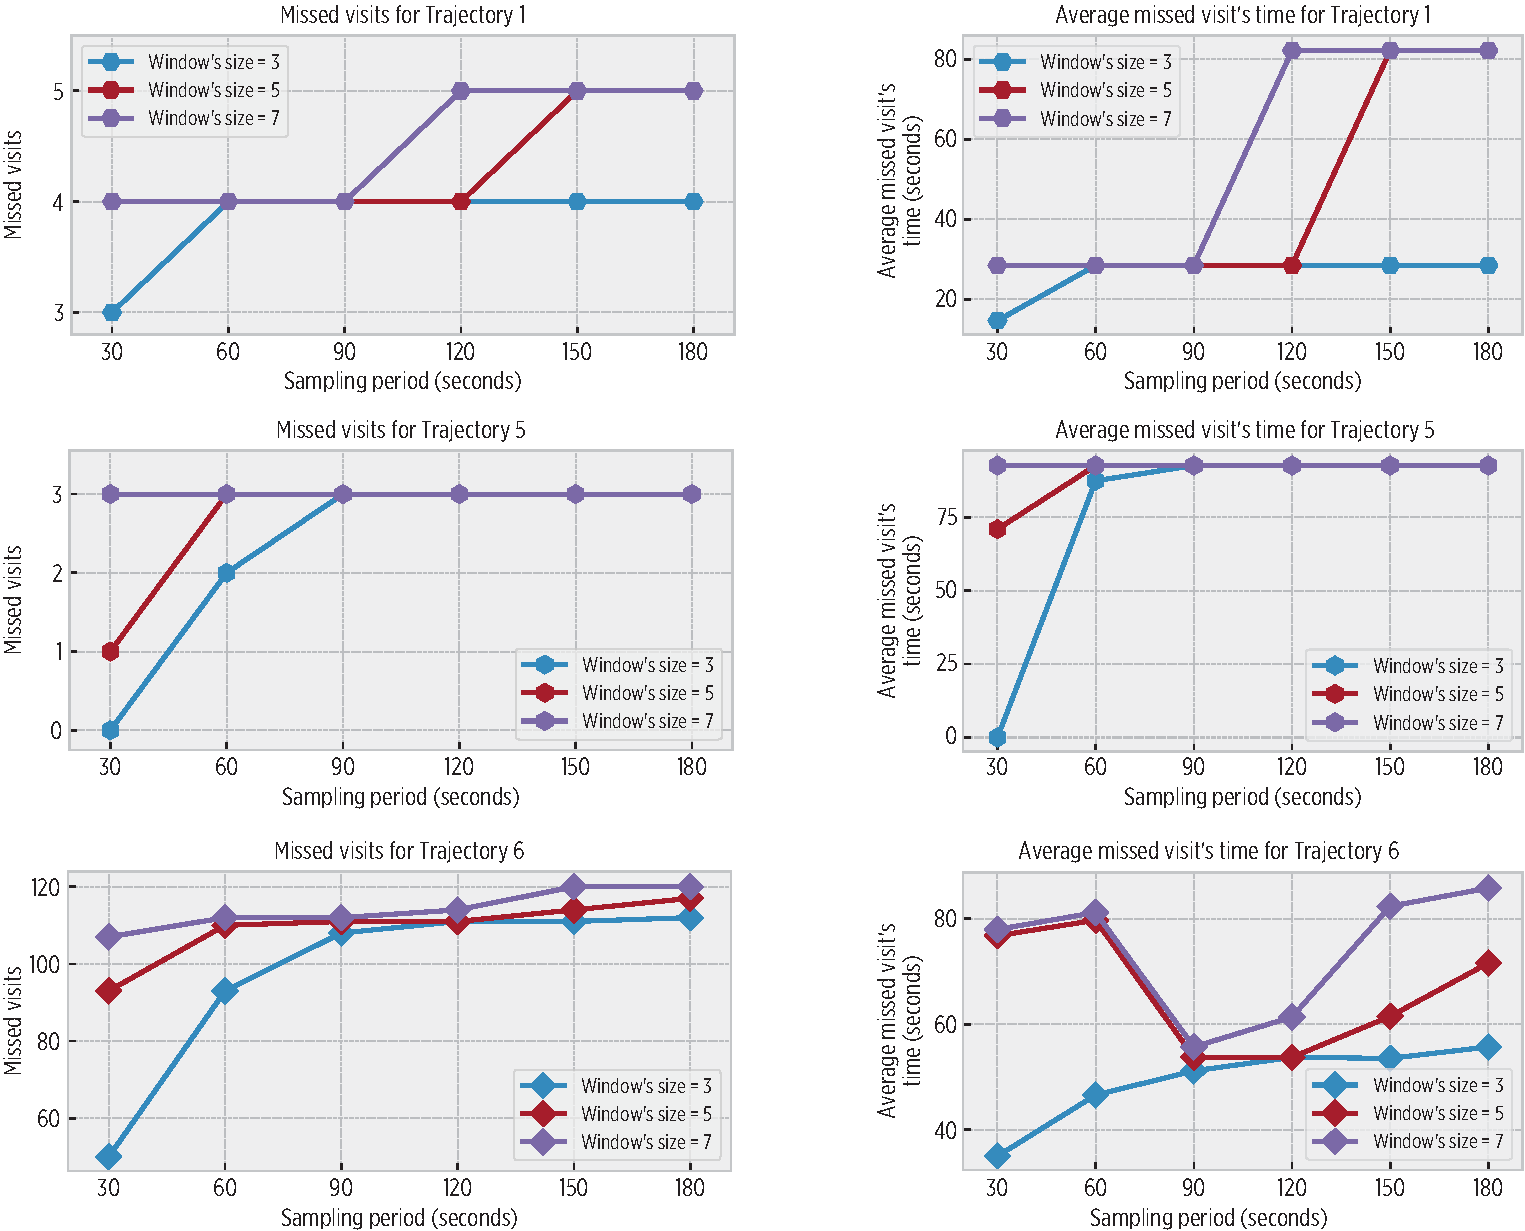
\includegraphics[width=0.78\textwidth]{vectors/exp-2-visits-for-slides}
%   \caption{Visits missed by the \emph{Geofencing} module for each combination of sampling period and window size values. The largest amount is obtained for the \emph{Trajectory 6}, given its length (more than 30 days). Nevertheless, they do not account for a considerable time in overall trajectories.}
% \end{figure}
% \end{frame}


% \begin{frame}[noframenumbering]{Preliminary experimentation}{Holistic evaluation: Results}
% \small 
% \vspace{-0.5cm}
% {
%   \centering
%   \includegraphics[width=0.7\textwidth]{vectors/exp-4-sigmoid-header-top-row}
%   \par 
% }

% \begin{columns}
% \begin{column}[T]{0.48\textwidth}
% \begin{block}{\small \textbf{Arrival latency}}
% {
%   \centering
%   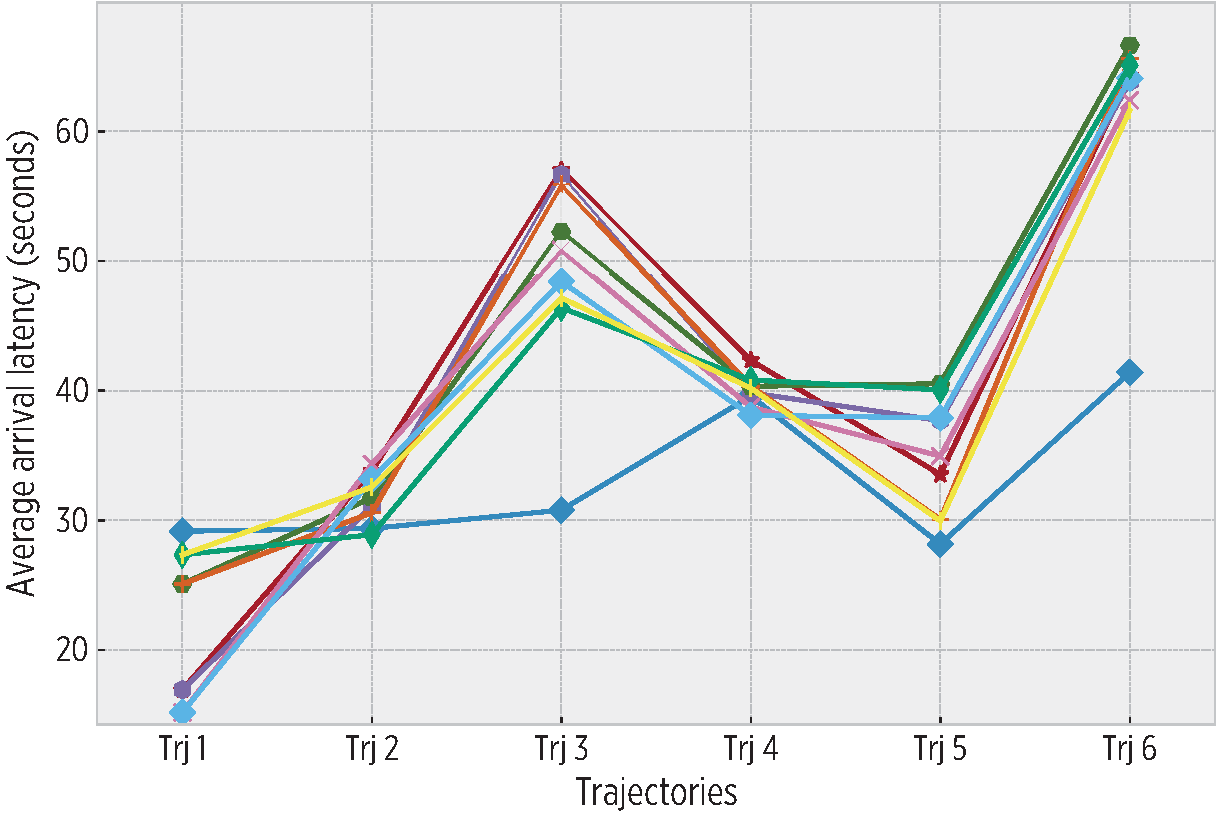
\includegraphics[width=\textwidth]{vectors/exp-4-arrival-latency-for-slides-v2}
%   \captionof{figure}{Arrival latency observed by the platform in experimental trials. The largest average value is below 65 seconds, explained by the fact that 2 location updates must be collected by the \emph{Geofencing} module before identifying an arrival event.}
%   \par 
% }
% \end{block}
% \end{column}

% \begin{column}[T]{0.52\textwidth}
% \begin{block}{\small \textbf{Departure latency}}
% {
%   \centering
%   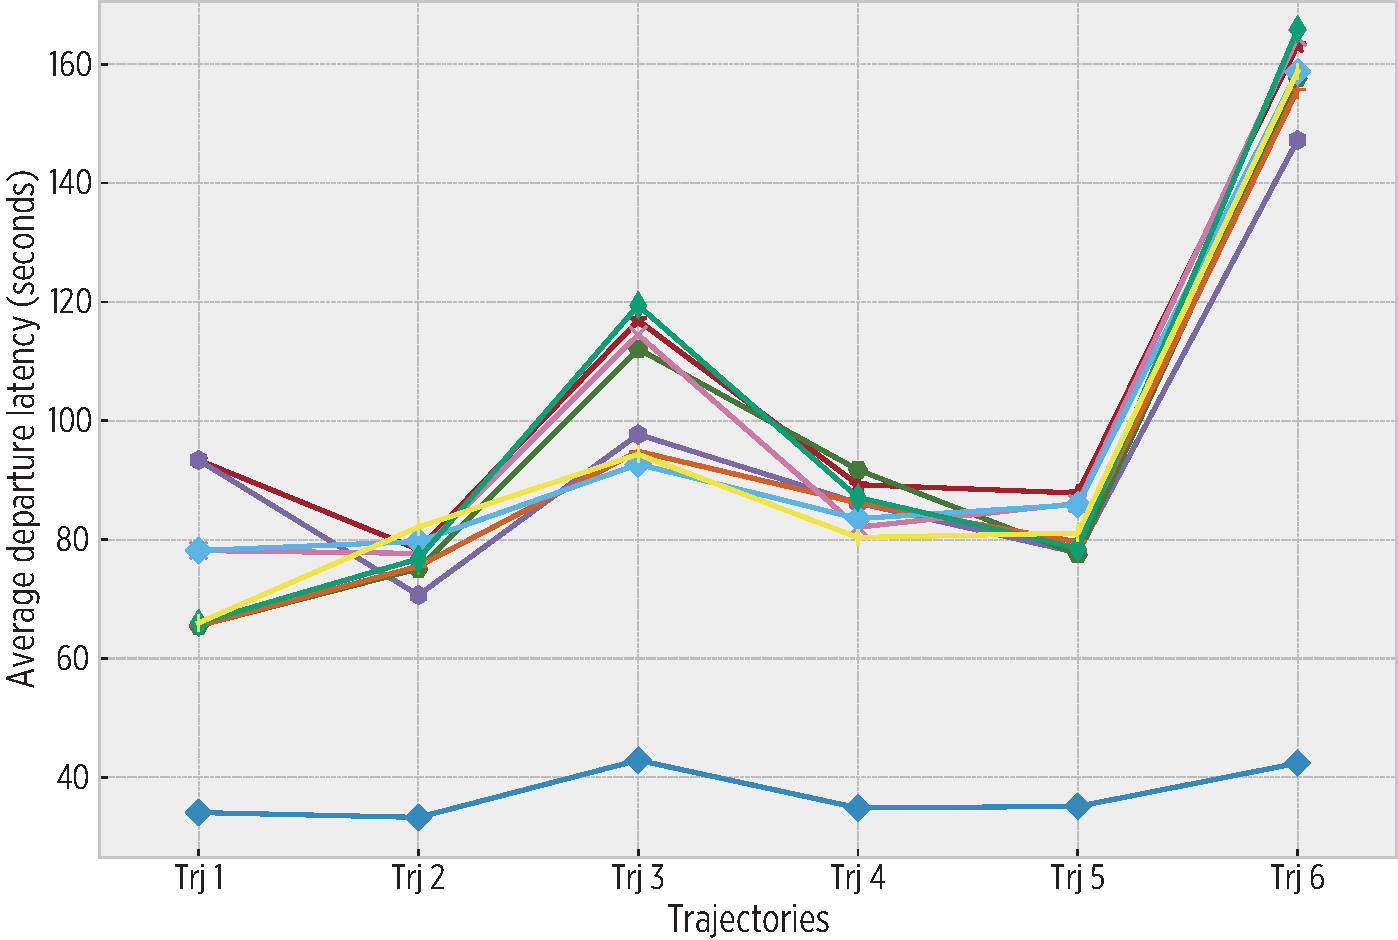
\includegraphics[width=\textwidth]{vectors/exp-4-departure-latency-for-slides-v2}
%   \captionof{figure}{Departure latency observed by the platform across performed experimental trials. The latencies are within 65 and 165 seconds, which is aligned with the different values specified to the CC for its sigmoid-driven sampling.}
%   \par
% }
% \end{block}
% \end{column}
% \end{columns}
% \end{frame}

% \begin{frame}[noframenumbering]{Preliminary experimentation}{Holistic evaluation: Results}
% \small
% \vspace{-0.5cm}
% {
%   \centering
%   \includegraphics[width=0.7\textwidth]{vectors/exp-4-sigmoid-header-top-row}
%   \par 
% }

% \begin{columns}
% \begin{column}[T]{0.5\textwidth}

% \begin{block}{\small \textbf{Trajectory distance difference}}
% {
%   \centering
%   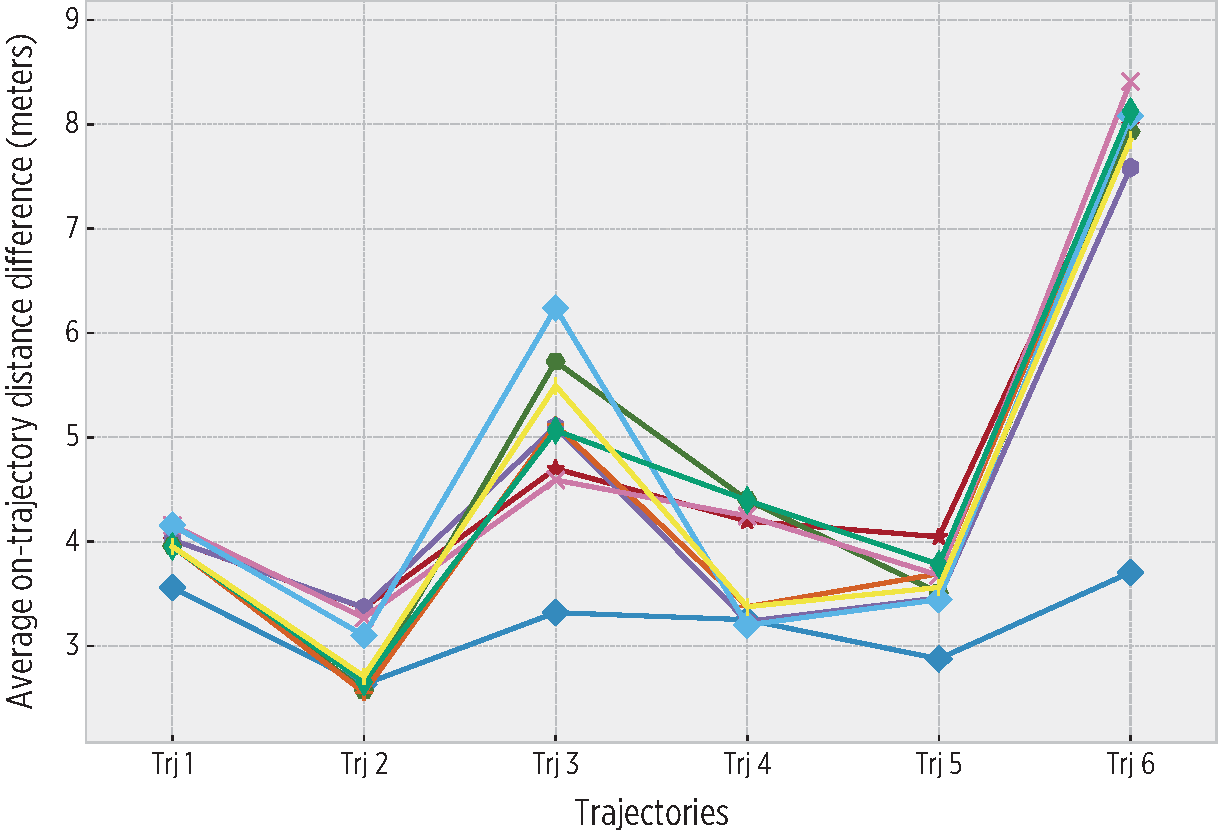
\includegraphics[width=\textwidth]{vectors/exp-4-on-trajectory-distance-for-slides-v2}
%   \captionof{figure}{The average distance of equivalent trajectory segments during experimental trials. The values are enclosed within $2.5~m$ and $8.5~m$, with the 30 seconds sampling obtaining the lowest values in each trial.}
%   \par
% }
% \end{block}

% \end{column}

% \begin{column}[T]{0.5\textwidth}
% \begin{block}{\small \textbf{Overall reduction of location update requests}}
% {
%   \centering
%   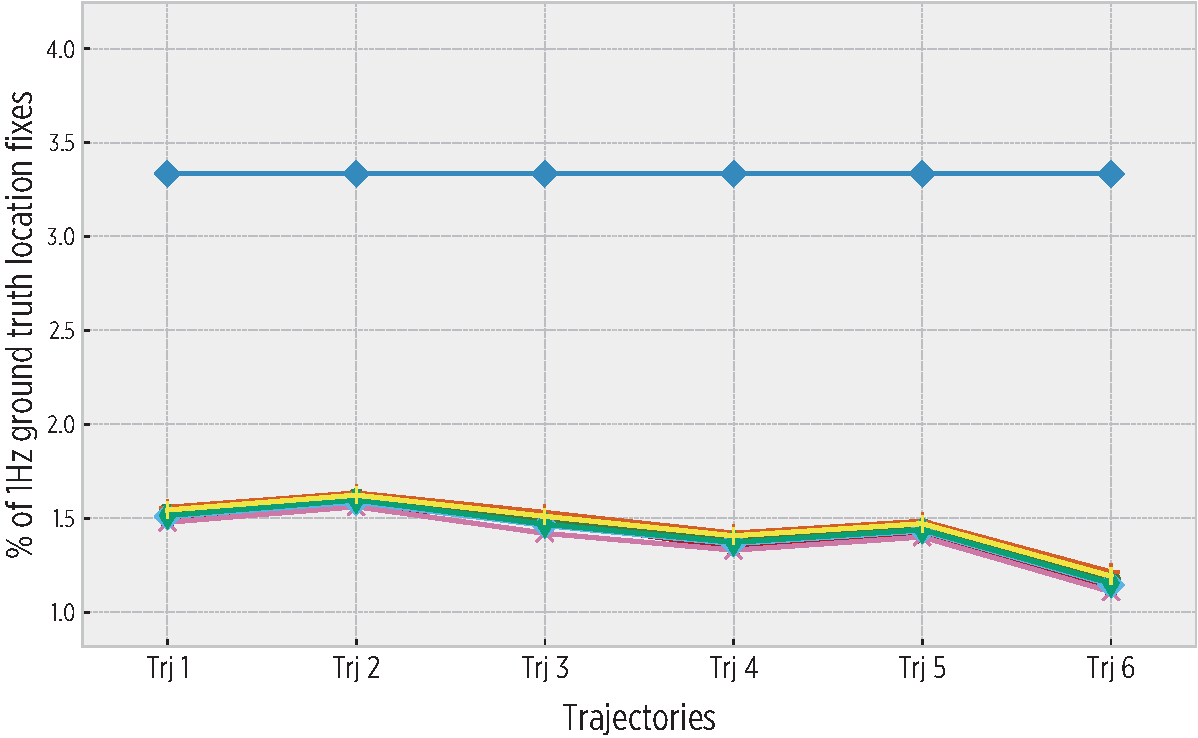
\includegraphics[width=\textwidth]{vectors/exp-4-location-requests-for-slides-v2}
%   \captionof{figure}{The proportion of location update requests employed by each experimental trial with respect to the corresponding $1~Hz$ ground truth trajectory. All of the parameter combinations outperform the 30 seconds sampling period, which provides a rough estimation of the energy savings that the system could achieve in on-device implementations.}
%   \par
% }
% \end{block}
% \end{column}
% \end{columns}
% \end{frame}

% \begin{frame}[noframenumbering]{Preliminary experimentation}{Energy saving expectations of on-device stay points detection}
% \small
% % \vspace{-0.5cm}
% \begin{columns}
% \begin{column}{0.55\textwidth}
% \begin{block}{\small \textbf{Description}}
% \begin{itemize}
%   \item This experiment explored whether a smartphone could detect stay points by itself, and the energy savings of such implementation with respect of typical Mobile Cloud Computing (MCC) based solutions.
%   % \item Typical solutions implement a Mobile Cloud Computing (MCC) approach on which the smartphone only collects and offloads the processing to external servers.
% \end{itemize}
% \end{block}
% \end{column}

% \begin{column}{0.4\textwidth}
% \begin{table}
% \centering
% \renewcommand{\arraystretch}{0.8}
% \resizebox{0.95\textwidth}{!}{%
% \begin{tabular}{lll}
% \toprule
% \multirow{2}{*}{\textbf{Stay Points Detector}} & \textbf{Time threshold} ($\delta_{time}$): & $45~min$ \\
% \cmidrule[0.25pt]{2-3}
%  & \textbf{Distance threshold} ($\delta_{distance}$): & $500~m$ \\

% \cmidrule[0.25pt]{1-3}
% \textbf{Sampling periods}: & \multicolumn{2}{l}{30, 60, 90, 120, 150 seconds} \\
% \bottomrule
% \end{tabular}
% }
% \caption{Input parameters for the energy saving expectations of on-device stay points detection experiment.}
% \end{table}
% \end{column}
% \end{columns}

% \begin{figure}
%   \centering
%   \includegraphics[width=\columnwidth]{vectors/plot-energy-performance-r2-for-slides}
%   \caption{Energy performance comparison of on-device vs. MCC sample apps using different GPS sampling periods. Each of the on-device trials last longer than its corresponding remote implementation.}
% \end{figure}

% \end{frame}


% \begin{frame}[noframenumbering]{Preliminary experimentation}{Energy consumption of fixed-sampling periods: Results}
% \vspace{-0.4cm}
% {
%   \centering
%   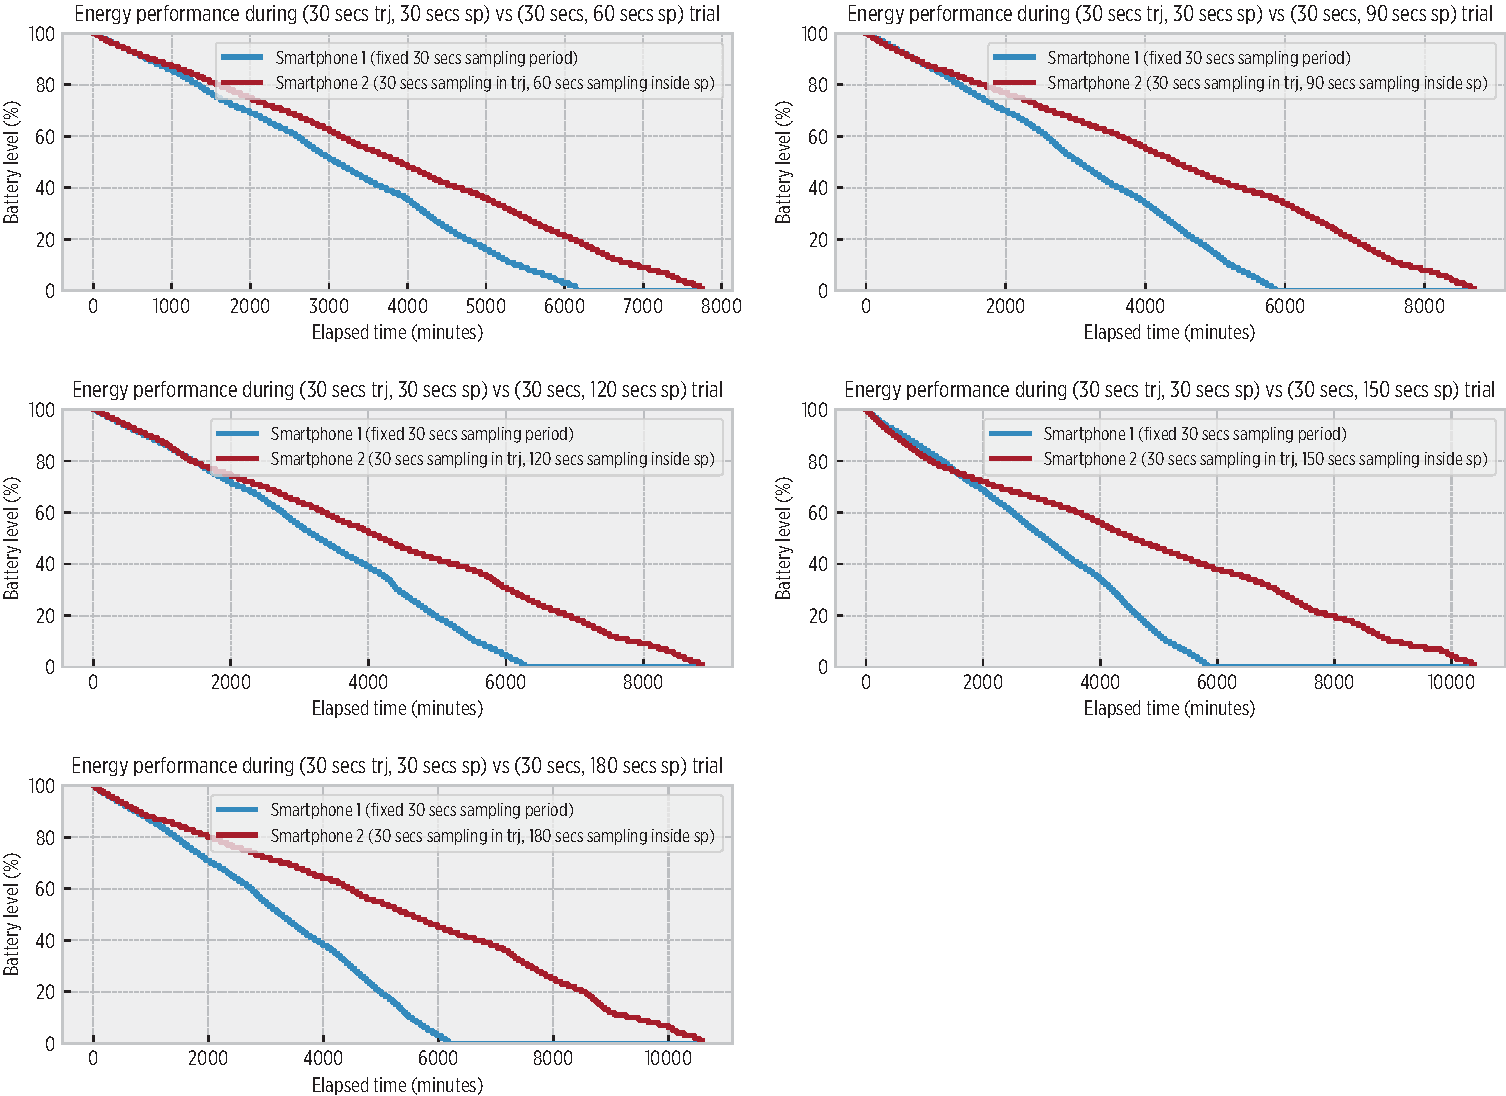
\includegraphics[width=0.85\textwidth]{vectors/exp-6-energy-burnout}
%   \captionof{figure}{Energy performance of a fixed 30 seconds sampling versus a basic sampling adaptation consisting in a 30 seconds sampling in trajectory mode and a slower sampling rate during stay point mode. The separation between the lines in each plot starts after the system learns the stay points with the largest weight in user mobility (home and work places).}
%   \par
% }
% \end{frame}


% \begin{frame}[noframenumbering]{Preliminary experimentation}{Energy consumption of fixed-sampling periods: Results}
% \vspace{-0.4cm}
% {
%   \centering
%   %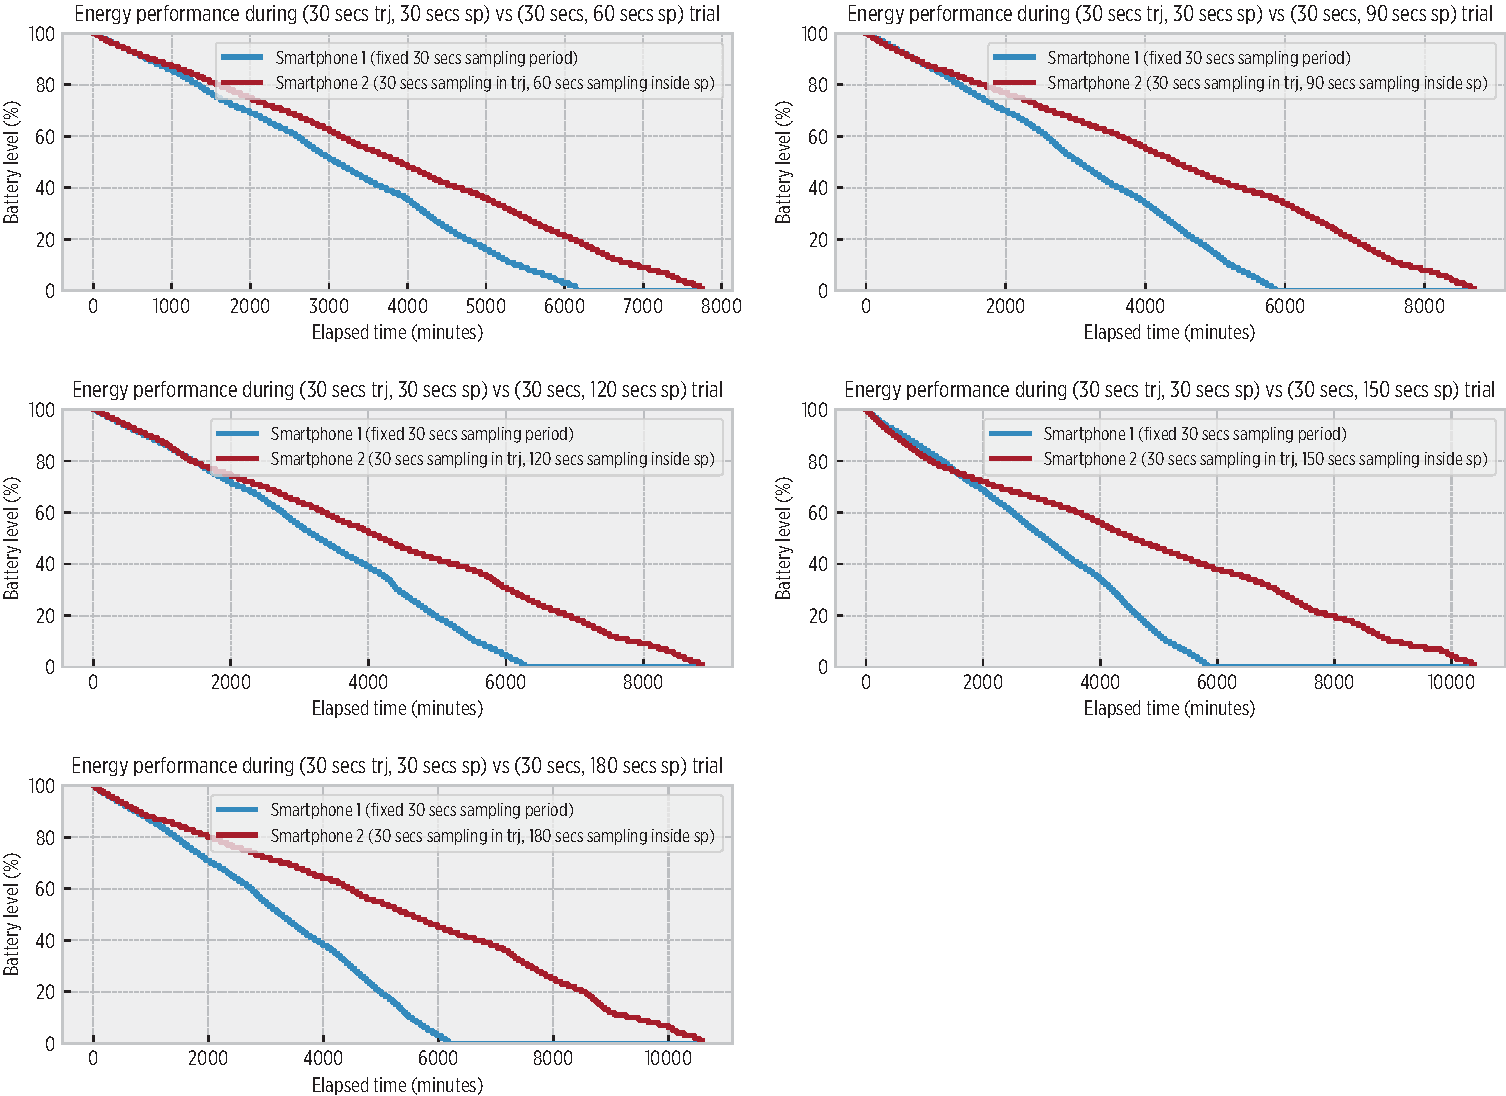
\includegraphics[width=0.85\textwidth]{vectors/exp-6-energy-burnout}
%   %\captionof{figure}{Energy performance of a fixed 30 seconds sampling versus a basic sampling adaptation consisting in a 30 seconds sampling in trajectory mode and a slower sampling rate during stay point mode. The separation between the lines in each plot starts after the system learns the stay points with the largest weight in user mobility (home and work places).}
%   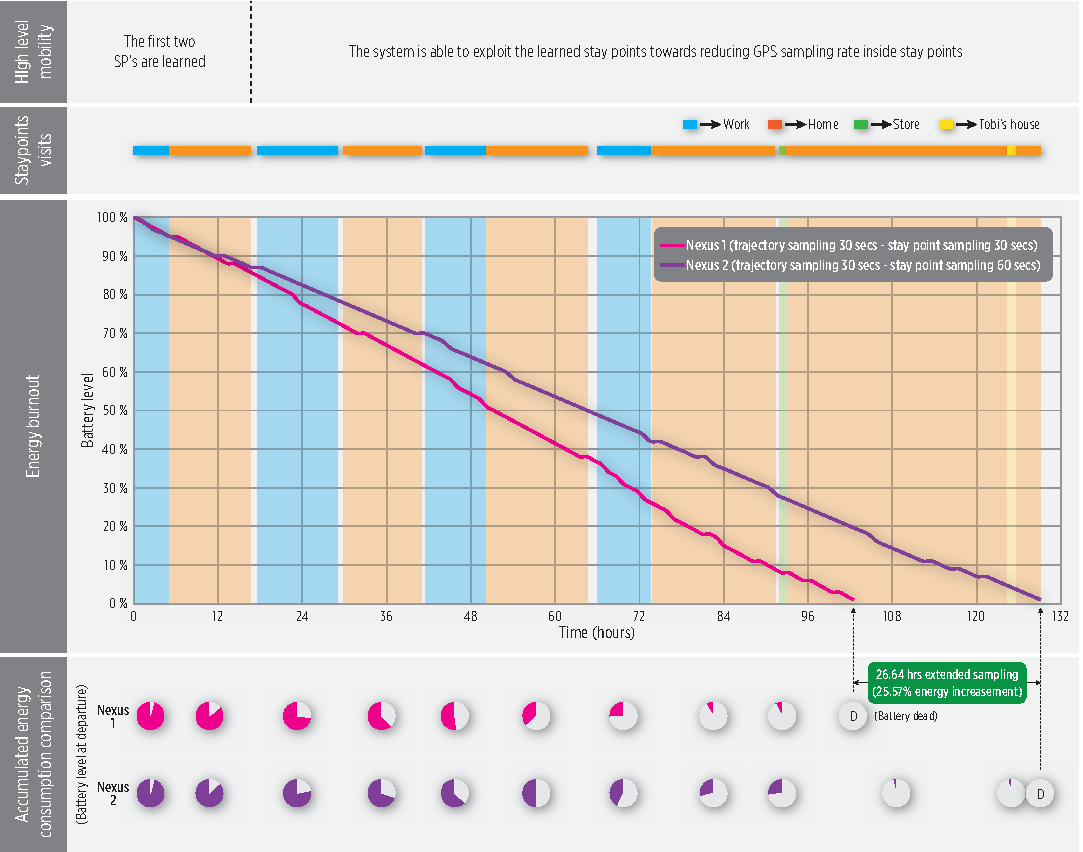
\includegraphics[width=0.8\textwidth]{vectors/energy-results-v2}
%   \captionof{figure}{Energy performance obtained by the CDS along the mobility described by user (trial corresponding to the 30 seconds in trajectory and 60 seconds in stay point sampling).}
%   \par
% }
% \end{frame}

% \begin{frame}[noframenumbering]{Preliminary experimentation}{Energy consumption of fixed-sampling periods: Results}
% \begin{figure}
%   % 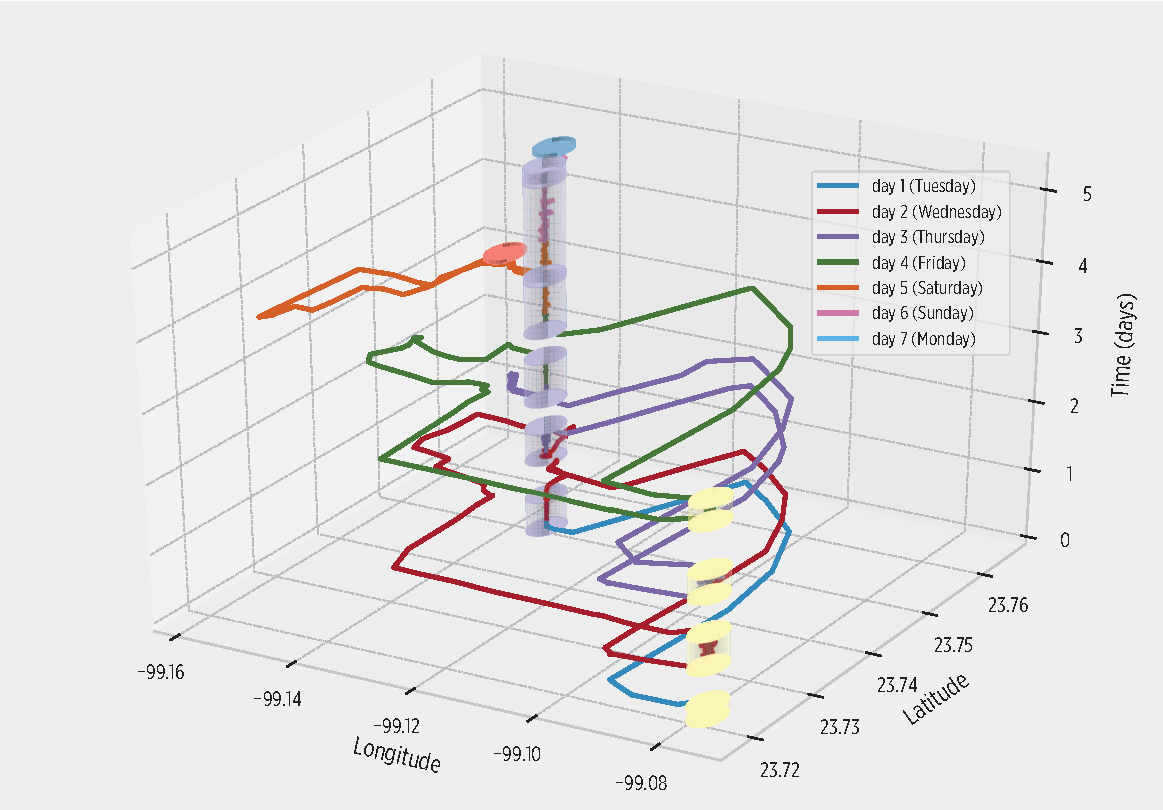
\includegraphics[width=0.8\textwidth]{vectors/exp-6-map-trj-4-adaptive-sampling-60-sp}
%   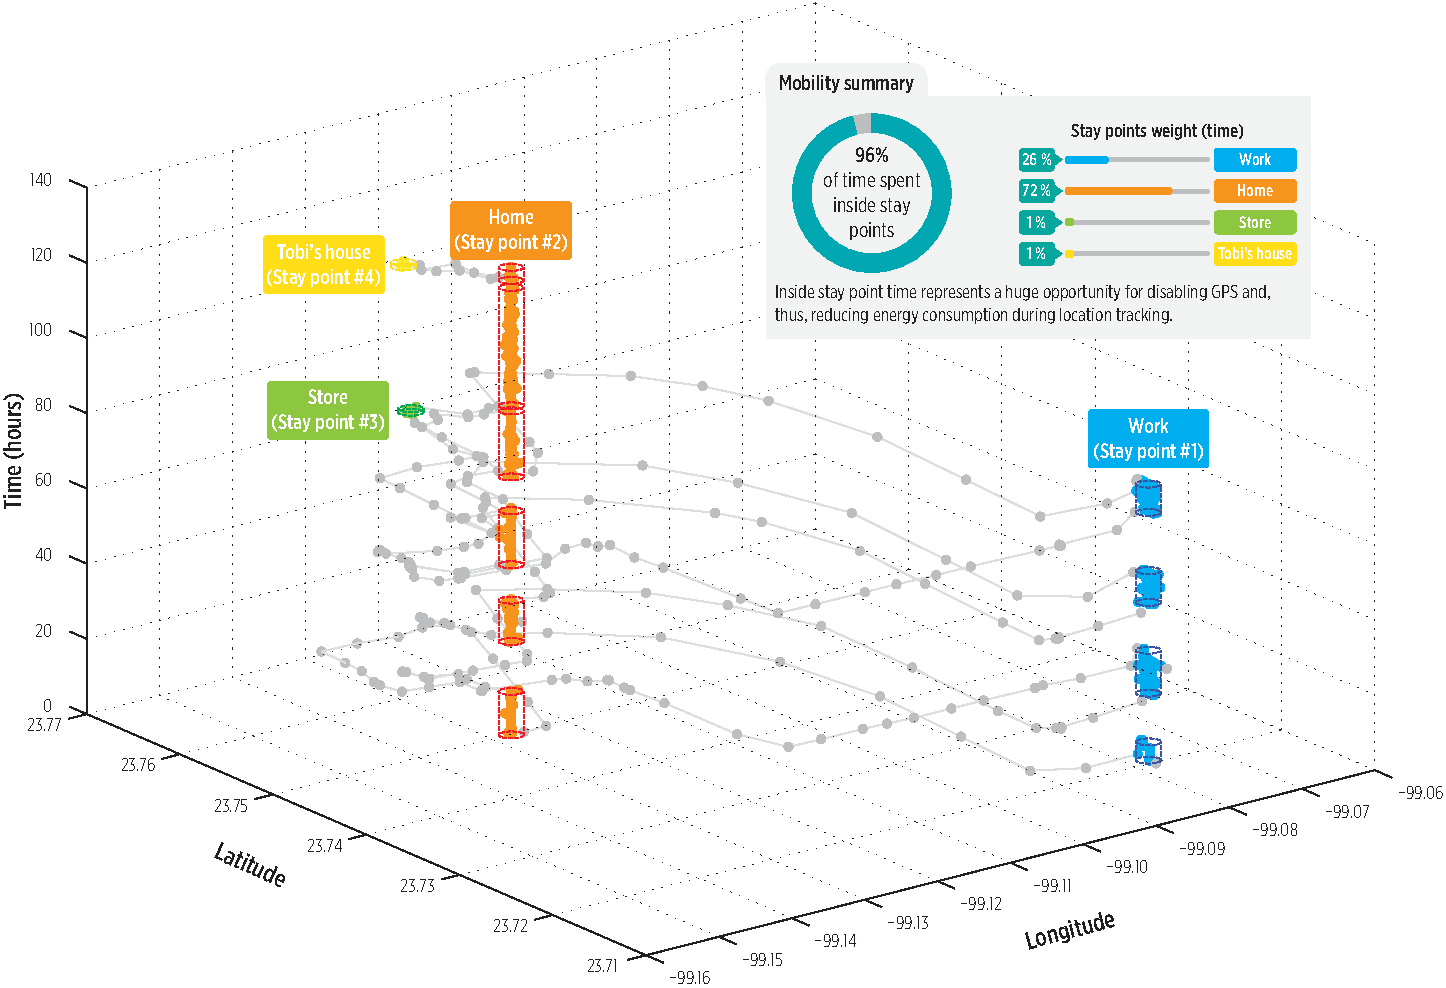
\includegraphics[width=0.85\textwidth]{vectors/stay-points-as-3d-v2}
%   \caption{The stay points and visits identified by the system, as well as the mobility summary obtained from such information (trial corresponding to the 30 seconds in trajectory and 60 seconds in stay point sampling).}
% %  \caption{The information autonomously learned by the STM during the trial corresponding to the 30 seconds in trajectory and 60 seconds in stay point sampling scheme. The height of cylinders corresponds with the stay time during each stay point visit.}
% \end{figure}
% \end{frame}


\end{document}
